% This is LLNCS.DEM the demonstration file of
% the LaTeX macro package from Springer-Verlag
% for Lecture Notes in Computer Science,
% version 2.4 for LaTeX2e as of 16. April 2010
%
\documentclass{elsarticle}

%
\usepackage{makeidx}  % allows for indexgeneration
\usepackage{pstricks}
%\usepackage{auto-pst-pdf}
\usepackage{lscape}
\usepackage{hyperref}
%\usepackage[cp850]{inputenc}
\usepackage{amsmath, amssymb}
\usepackage{enumerate}
\usepackage{latexsym,makeidx,graphicx,color,colortbl}
\usepackage{moreverb,amsmath,amssymb}
\usepackage[latin1]{inputenc}
\usepackage{tabulary}
\usepackage{multicol}
\usepackage{pdflscape}
\usepackage{boxedminipage}
\usepackage{subfig}
\usepackage{epsfig}
\usepackage{pdfpages}
\usepackage{arydshln}
\usepackage{epstopdf}
\usepackage{setspace}
\pagestyle{plain}
\parindent 0.5cm
\parskip=0cm
\renewcommand{\comment}[1]{}
\newcommand{\entero}{\mathbb{Z}}
\ifx\theorem\NoDefinido
  \newcommand{\ComaMat}{}
  \newcommand{\PuntoMat}{}
  \newtheorem{theorem}{Theorem}[section]
  \def\thetheorem{\thesection.\arabic{theorem}}
  \newtheorem{definition}[theorem]{Definition}
  \newtheorem{conjetura}[theorem]{Conjecture}
  \newtheorem{proposition}[theorem]{Proposition}
  \newtheorem{corollary}[theorem]{Corollary}
  \newtheorem{lemma}[theorem]{Lemma}
  \newtheorem{fact}[theorem]{Fact}
  \newtheorem{example}[theorem]{Example}
\fi
\newenvironment{prueba}{\noindent {\it Proof: }}{\qed}
\newenvironment{skecht}{\noindent {\it Proof (sketch): }}{\qed}


\newcommand{\bdfn}{\begin{definition} \begin{rm}}
\newcommand{\edfn}{\end{rm}$ $\qed \end{definition}}
%\newcommand{\bdfn}{\begin{definition} \begin{rm}}
%\newcommand{\edfn}{\vspace{-2ex}
%{\flushright $\Box$\\
%\mbox{}\vspace{-2ex}
%} \end{rm} \end{definition}}
\newcommand{\bthm}{\begin{theorem} \begin{rm}}
\newcommand{\ethm}{\vspace{-4ex}{\flushright $\Box$\\
\mbox{}\vspace{-4ex}} \end{rm} \end{theorem}}
\newcommand{\bprop}{\begin{proposition} \begin{rm}}
\newcommand{\eprop}{\vspace{-4ex}{\flushright $\Box$\\
\mbox{}\vspace{-4ex}} \end{rm} \end{proposition}}
\newcommand{\bcor}{\begin{corollary}\begin{rm}}
\newcommand{\ecor}{\vspace{-4ex}{\flushright $\Box$\\
\mbox{}\vspace{-4ex}} \end{rm} \end{corollary}}
\newcommand{\blem}{\begin{lemma} \begin{rm}}
\newcommand{\elem}{\vspace{-4ex}{\flushright $\Box$\\
\mbox{}\vspace{-4ex}} \end{rm} \end{lemma}}
\newcommand{\bfact}{\begin{fact} \begin{rm}}
%\newcommand{\efact}{%\vspace{-4ex}{\flushright $\Box$\\
%\mbox{}%\vspace{-4ex}} \end{rm} \end{fact}}
%\newcommand{\bex}{\begin{example} \begin{rm}}
%\newcommand{\eex}{%\vspace{-2ex}{\flushright $\Box$\\
%\mbox{}2ex}} \end{rm} \end{example}}
%%
% signo menos con un punto encima
\newcommand{\menos}{\renewcommand{\arraystretch}{0.0002}
\begin{array}[b]{c}
\scriptstyle{.} \\
-
\end{array}\renewcommand{\arraystretch}{1.0}}

% simbolo de union
\newcommand{\union}[2]{\renewcommand{\arraystretch}{0.45}
\begin{array}{c}
{\scriptstyle #2}\\
\bigcup\\
{\scriptstyle #1}
\end{array}\renewcommand{\arraystretch}{1.0}}

% simbolo de union
\newcommand{\unions}[1]{\renewcommand{\arraystretch}{0.47}
\begin{array}[t]{c}
\bigcup\\
{\scriptstyle #1}
\end{array}\renewcommand{\arraystretch}{1.0}}

% simbolo de interseccion
\newcommand{\inter}[2]{\renewcommand{\arraystretch}{0.45}
\begin{array}{c}
{\scriptstyle #2}\\
\bigcap\\
{\scriptstyle #1}
\end{array}\renewcommand{\arraystretch}{1.0}}

%suma con cosas arriba y debajo
\newcommand{\suma}[2]{\renewcommand{\arraystretch}{0.42}
\hspace*{-0.1cm}
\begin{array}{c}
{\scriptstyle #2}\\
{\mbox{\huge $\Sigma$}}\\
{\scriptstyle #1}
\end{array}\hspace*{-0.1cm}\renewcommand{\arraystretch}{1.0}}

%suma con solo cosas abajo
\newcommand{\sumas}[1]{\renewcommand{\arraystretch}{0.42}
\hspace*{-0.1cm}
\begin{array}[t]{c}
{\mbox{\huge $\Sigma$}}\\
{\scriptstyle #1}
\end{array}\hspace*{-0.1cm}\renewcommand{\arraystretch}{1.0}}

% a con subrayado debajo �
\newcommand{\suba}{$\!~^{\underline{{\small a}}}~$}

% sumatorio
\newcommand{\sumad}[2]{\renewcommand{\arraystretch}{0.48}
\begin{array}[t]{c}
{\mbox {\huge $\Sigma$}}\\
{\scriptstyle #1}\\
{\scriptstyle #2}
\end{array}\renewcommand{\arraystretch}{1.0}}

\newcommand{\nat}{{\rm I\! N}}

% sumatorio triple
\newcommand{\sumat}[3]{\renewcommand{\arraystretch}{0.48}
\begin{array}[t]{c}
{\mbox {\huge $\Sigma$}}\\
{\scriptstyle #1}\\
{\scriptstyle #2}\\
{\scriptstyle #3}
\end{array}\renewcommand{\arraystretch}{1.0}}

% maximo con 1 parametro
\newcommand{\maximo}[1]{\renewcommand{\arraystretch}{0.40}
\begin{array}[t]{c}
max\\
{\scriptstyle #1}
\end{array}\renewcommand{\arraystretch}{1.0}}

\newcommand{\maximot}[1]{\renewcommand{\arraystretch}{0.40}
\begin{array}[t]{c}
max_{\leq_1}\\
{\scriptstyle #1}
\end{array}\renewcommand{\arraystretch}{1.0}}

% maximo con 2 parametros
\newcommand{\maximod}[2]{\renewcommand{\arraystretch}{0.45}
\begin{array}[t]{c}
max\\
{\scriptstyle #1}\\
{\scriptstyle #2}
\end{array}\renewcommand{\arraystretch}{1.0}}

% pila con menos distancia. Fila de abajo en peque\~{n}o
\newcommand{\pila}[2]{\renewcommand{\arraystretch}{0.48}
\begin{array}[t]{c}
#1\\
{\scriptstyle #2}
\end{array}\renewcommand{\arraystretch}{1.0}}

% precondicion
\newcommand{\precond}[1]{\hspace*{-0.4em}~^{\bullet}\hspace*{-0.05em}#1}




\begin{document}

\title{A Coloured Petri Net Approach to Model and 
Analyse Stateful Workflows Based on WS-BPEL and WSRF/WSN\tnoteref{t1}}
\tnotetext[t1]{Research partially supported by projects
TIN2009-14312-C02-02 and TIN2012-36812-C02-02.}



%\author{ Gregorio~D\'{\i}az~and~Ismael~Rodr\'{i}guez%
%\IEEEcompsocitemizethanks{\IEEEcompsocthanksitem Gregorio D�az is with the Department
%of Computer Science, University of Castilla-La Mancha, 02071, Albacete, Spain.\protect\\
%E-mail: gregorio.diaz@uclm.es \IEEEcompsocthanksitem Ismael Rodr�guez
%is with the Dept. Sistemas Inform�ticos y Computaci�n,
%Universidad Complutense de Madrid, 28040, Madrid, Spain.\protect\\
%E-mail: isrodrig@sip.ucm.es}
%\thanks{}}


\author{Jos\'e Antonio Mateo}
\ead{joseantonio.mateo@uclm.es}
\author{Valent�n Valero}
\ead{valentin.valero@uclm.es}
\author{Hermenegilda Maci�}
\ead{hermenegilda.macia@uclm.es}
\author{Gregorio D�az}%\corref{cor1}}
\ead{gregorio.diaz@uclm.es}

%\cortext[cor1]{Corresponding author}
%\cortext[cor2]{Principal corresponding author}
%\fntext[fn1]{This is the specimen author footnote.}
%\fntext[fn2]{Another author footnote, but a little more longer.}
%\fntext[fn3]{Yet another author footnote. Indeed, you can have
%any number of author footnotes.}


\address{Universidad de Castilla-La Mancha, Instituto de
Investigaci�n en Inform�tica, 02071, Albacete, Spain.} 


\begin{abstract}
Composite Web services technologies are widely used 
due to their ability to provide interoperability among services 
from different companies. Web services are usually \emph{stateless},
which means that no state is stored from the clients viewpoint. 
However, some new applications and services have emerged, which
require to capture the state of some resources. Thus,
new standards to model Web services states have appeared, 
such as Open Grid Services Infrastructure (OGSI), 
which became Web Services Resource Framework (WSRF). 
In this paper, we present a formal model based
on WS-BPEL and WSRF/WSN, and we provide a prioritised-timed coloured Petri net semantics for 
it. This semantics captures the main activities of WS-BPEL considering
also other important aspects, both from WS-BPEL and 
WSRF/WSN, such as fault and event handlers, time-outs and
the WS-Notification publish-subscribe system.
% to manage Cloud/Grid notifications.   
\end{abstract}
\maketitle

\section{Introduction}

The development of software systems is becoming more complex with the 
appearance
of new computational paradigms such as Service-Oriented  Computing  (SOC), 
Grid Computing and Cloud Computing.
In these systems, the service provider needs to ensure some levels of 
quality and privacy to the clients in a way that had never been considered. It is therefore necessary to develop new techniques to benefit from the advantages 
of recent approaches, such as Web service compositions. Formal models of concurrency have been widely used for the description and analysis of concurrent and distributed systems. 
Grid/Cloud environments are characterized by a dynamic environment due to the heterogeneity and volatility of resources. There are two complementary views to composite Web services: Choreography and Orchestration. The choreography view describes the observable interactions among services and can
be  defined  by  using  specific  languages such as Web  Services
Choreography  Description  Language  (WS-CDL) %\cite{WSCDL}
or  by
using more general languages like UML Messages Sequence
Charts (MSC). On the other hand, orchestration concerns
the internal behaviour of a Web service in terms of invocations
to  other  services.  Web Services Business Process Execution Language (WS-BPEL) \cite{BPEL4WS} is normally used 
to describe Web service orchestrations, so this
is considered the de-facto standard language for describing Web services
workflows in terms of Web service compositions.

To facilitate additional interoperability among services, more standardization is required to deal with distributed resources. In January of 2004, several members of the \emph{Globus Alliance} organization and the computer multinational \emph{IBM} with the help of experts from companies such as \emph{HP, SAP, Akamai, etc.} defined the basis architecture and the initial specification documents of a new standard for that purpose, Web Services Resource Framework (WSRF)~\cite{Banks2006,Czajkowski2004,Foster2004}. Although the Web service 
definition does not consider the notion of state, interfaces frequently provide the user with the ability to access and manipulate
states, that is, data values that persist across, and evolve as a result of Web service interactions. The messages that the services 
send and receive imply (or encourage programmers to infer) the existence of an associated stateful resource. It is then desirable 
to define Web service conventions to enable the discovery of, introspection on, and interaction with stateful resources in standard 
and interoperable ways. In addition, the WS-Notification (WSN) family of specifications defines the Web Services standard approach to send and receive
notifications. Thus, WSN can be used in conjunction with WSRF to model a publish/subscribe architecture, thus allowing clients to subscribe to distributed WS-Resources and being notified in the case that this subscription condition holds or the state of that resource changes.

The main motivation of this work is to provide a formal 
semantics for WS-BPEL+WSRF/WSN to manage stateful Web services workflows 
by using the existing machinery in distributed systems,
and specifically a well-known formalism, such as coloured
Petri nets extended with time and priorities, which are a graphical model, but they also
provide us with the ability to simulate and analyse the modelled
system.

Thus, our aim is not to provide just another WS-BPEL semantics. 
In order to deal with the integration of WS-BPEL plus WSRF/WSN in a proper way, 
we have realised that it is more convenient 
to introduce a specific semantic model, which  covers 
properly all the relevant aspects of WSRF such as notifications and 
resource time-outs. 
The integration of WS-BPEL and WSRF/WSN is not new; in the literature, 
there are a bundle of works defining this integration, although 
none of these works define a formal semantics in terms of Petri
nets. In the next section we present an overview
of these works. 
However, we have considered that the integration of WSRF/WSN, and specifically the
time constraints that are inherent in this service language, would be captured
in a better way in a specific language, in which the main activity constructions
of WS-BPEL are considered, as well as a model for event and fault handling. 
%Nevertheless, to the best of our 
%knowledge, this is the first paper that uses coloured Petri nets to 
%model both approaches allowing designers to validate and 
%verify their models before starting the implementation with the 
%corresponding benefits. We have also defined the necessary Petri 
%nets to model and verify WSRF Publish/Subscribe system to 
%standardise the way of managing subscriptions in Cloud systems. 
%These observations motivated the advent of the WS-Resource approach to modeling states in Web services.
%A WS-Resource is defined as the composition of a Web service and a stateful resource that is (i) expressed as an association of a XML document with 
%defined type with a portType, and (ii) addressed and accessed according to the implied resource pattern, a conventional use
%of WS-Addressing endpoint references (EPR). In the implied resource pattern, a stateful resource identifier is encapsulated in an 
%endpoint reference and used to identify the stateful resource to be used in the execution of a Web service message 
%exchange. 
%An Endpoint Reference shall consist of: Uniform Resource Identifier (URI), parameters of the message being sent to request the sending of the Endpoint Reference and data on the interface used. In this exchange, the resource identifier is encapsulated in an Endpoint Reference used to identify the resource in any exchange of messages between services which belongs to the choreography. 

%We then define an integrated language, which is based on BPEL, but including many aspects of WSRF. There are many different works that formalize the main constructions of WS-BPEL. In the related section work we show a brief description of some of these works.
%However, we have considered that the integration of WSRF, and specifically the
%time constraints that are inherent in this service language, would be captured
%in a better way in a specific language, in which the main activity constructions
%of WS-BPEL are considered, as well as a model for event and fault handling. 
%We can see a WS-Resource as a collection of properties \emph{P} identified by an address \emph{EPR} with an associated \emph{timeout}. This timeout represents the WS-Resource lifetime. Without loss of generality, we have reduced the resource properties set to only one allowing us to use the resource identifier \emph{EPR} as the representative of this property. As well, in BPEL, we have taken into consideration the root scope only, avoiding thus any class of nesting among scopes, and we have considered the event and fault handling, leaving the other handling types as future work. The rest of the paper is organized as follows. In Section \ref{relwork}, we present the basic concepts to understand this paper and some related works. Finally, Section \ref{conclu} finishes the paper giving some conclusions and possible future works.   


\section{Background and Related Work}\label{relwork}

In this Section, we provide an overview of  WS-BPEL and WSRF/WSN,
and we also review some related works.

\subsection{Overview of WS-BPEL/WSRF/WSN}\label{BPEL/WSRF}

WS-BPEL \cite{BPEL4WS}, for short BPEL, 
is an OASIS orchestration language for specifying actions within 
Web services business processes. WS-BPEL is therefore an orchestration
language in the sense that it is used to define the composition
of services from a local viewpoint, describing the individual
behaviour of each participant. More specifically, WS-BPEL is a language for describing the behaviour of a business process based on interactions between the process and its partners. At the core of the WS-BPEL process model is the notion of peer-to-peer interaction between services described in Web Services Description Language (WSDL), both the process and its partners are exposed as WSDL services. Thus, a business process defines how to coordinate the interactions between a process instance and its partners through Web Service interfaces, whereas the structure of the relationship at the interface level is encapsulated in what is called a \emph{partnerLink}. These are instances of typed connectors which specify the WSDL port 
types the process offers to and 
requires from a partner at the other end of the partner link. A port type  defines the connection point to a web service defining a named set of abstract operations and the abstract messages involved. 

In particular, 
we will consider a composite Web service consisting of a set of 
orchestrators, described by BPEL+WSRFN syntax, which
exchange messages through some communication channels ({\em partnerLinks}). Moreover, WS-BPEL processes use {\em variables} to temporarily store 
data. Variables are therefore declared on a process or on a scope 
within that process. In our case, there will be a single scope
({\em root}), so no nesting is considered in our framework.
Besides, for simplicity again, we will only consider integer
variables.

An orchestrator consists of a main activity, representing
the normal behaviour of this participant. There are also
event and fault activities, which are executed upon the
occurrence of some events, or due to some execution failures,
respectively. WS-BPEL activities 
can be \emph{basic} or \emph{structured}. 
\emph{Basic activities} are those which describe the elemental 
steps of the process behaviour, such as the assignment of
variables ({\em assign}), empty action ({\em empty}), 
time delay ({\em wait}), invoke a service ({\em invoke}) and receive
a message ({\em receive}), reply to a client ({\em reply}),
and throw an exception ({\em throw}). We also have an action to {\em terminate}
the process execution at any moment ({\em exit}).
For technical reasons we have also included an additional activity {\em $\overline{reply}$}, which is used when a service invocation
expects a reply, in order to implement the synchronization with
the {\em reply} action from the server.  

\emph{Structured activities} encode control-flow logic in a nested
way. The considered structured activities are the following:
a {\em sequence} of activities, separated by a semicolon, 
the parallel composition, represented by two parallel bars ($\|$),
the conditional repetitive behaviour ({\em while}),
and a timed extension of the receive activity, which allows to
receive different types of messages with a time-out associated
({\em pick}).

WSRF~\cite{Banks2006} is a specification language 
developed by OASIS and some of the most pioneering computer companies, 
whose purpose is to define a generic framework for modelling Web services 
with stateful resources, which has been proposed to 
fully fit the OpenGrid Services
Infrastructure (OGSI) into the Web services stack, thus allowing Web service middleware to
be the base for Grid environments. The two main concepts behind the resource framework are 
WS-Resources and the implied resource pattern \cite{Leymann:2006}.


On the one hand, we can see a WS-Resource as a collection of properties \emph{P} identified by an address \emph{EPR} with an associated \emph{timeout}. This timeout represents the WS-Resource lifetime. Without loss of generality, we have reduced the resource properties set to only one allowing us to use the resource identifier \emph{EPR} as the representative of this property. On the other hand, the implied resource pattern specifies how to identify this resource.
It is based on the WS-Addressing~\cite{wsaddressing} specification and describes how a data
structure (EPR) is used for the identification of a WS-Resource.
Next, we describe the WSRF elements
that are considered in the BPEL+WSRFN framework:

\vspace*{-0.15cm}

%{\renewcommand{\arraystretch}{0.85}
%\begin{table}[!h]
%\begin{center}
%\begin{tabular}{|p{3.5cm}|p{8.5cm}|}
%\hline
%\cellcolor[gray]{.9}~ & \cellcolor[gray]{.9}~ \\
%\rowcolor[gray]{.9}
%\multicolumn{1}{>{\rowcolor[gray]{.9}}c|}{WS-CDL Syntax} & Metamodel\\
%\cellcolor[gray]{.9}\hspace*{1.5cm}Name & \cellcolor[gray]{.9}\hspace*{3.5cm}Describes\\
%\cellcolor[gray]{.9}~ & \cellcolor[gray]{.9}~ \\

%\begin{center}
%\vspace{-0.1cm}
%{\bf WS-ResourceProperties} 
%\end{center}
%& 
%\begin{flushleft}
%\vspace{-0.1cm}
%\hspace{0.3cm} WSRF uses a precise specification to define the properties of the WS-Resources.\\
%\end{flushleft}\\
%\hline

%\begin{center}
%\vspace{-0.1cm}
%{\bf WS-Basefaults} 
%\end{center}
%& 
%\begin{flushleft}
%\vspace{-0.1cm}
%\hspace{0.1cm} To standardize the format for reporting error messages.
%\\[-0.2cm]
%\end{flushleft}\\
%\hline

%\begin{center}
%\vspace{-0.1cm}
%{\bf WS-ServiceGroup} 
%\end{center}
%& 
%\begin{flushleft}
%\vspace{-0.25cm}
%\hspace{0.3cm} This specification allows the programmer to create groups that share a common set of properties.
%\end{flushleft}\\[-0.2cm]
%\hline

%\begin{center}
%\vspace{-0.2cm}
%{\bf WS-ResourceLifetime}
%\end{center}
%& 
%\begin{flushleft}
%\vspace{-0.4cm}
%\hspace{0.3cm} The mission of this specification is to standardize the process of destroying a resource and identify mechanisms 
%to monitor its lifetime. 
%\end{flushleft}\\[-0.2cm]
%\hline

%\begin{center}
%\vspace{0.4cm}
%{\bf WS-Notification}
%\end{center}
%& 
%\begin{flushleft}
%\vspace{-0.2cm}
%\hspace{0.3cm} This specification allows a \emph{NotificationProducer} to send \emph{notifications} 
%to a \emph{NotificationConsumer} in two ways: without following any formalism or with a predefined formalism.
%\end{flushleft}\\%[-0.1cm]
%\hline

%\end{tabular}
%\end{center}
%\caption{\label{tabla}WSRF main elements}
%\end{table}
%\vspace{-0.5cm}
\begin{itemize}
\item {\bf WS-ResourceProperties}: There is a precise specification 
to define WS-Resource properties, based on 
a Resource Properties Document (RPD),  which
defines the properties of the associated resource
(disk size, processor capacity, \ldots). 
Resources are identified by their EPRs,
so we will also use this mechanism for identification purposes,
but, for simplicity, we will consider these references as static, instead
of assuming a dynamic mechanism to assign them.
As a shorthand notation, EPRs will also be used to denote
the resource property values.

Furthermore,
a WSDL file must be provided in order to
facilitate the allowed resource operations.
Among the operations allowed by the standard are \emph{GetResourceProperty} 
and \emph{SetResourceProperty}, which are used to manipulate 
the resource property values.
%
%The developer 
%typically uses a Web service interface defined by others, so a 
%method to standardise the format for reporting error messages 
%facilitates the work.
%
%
\item {\bf WS-ResourceLifetime}: The WSRF specification does not 
provide a standard way to create resources. However,
resources have an associated lifetime, which means that once
this time has elapsed, the resource is considered to be destroyed,
and the subscribers could be notified.
%
We have then included, for completeness, an operation to create
resources, {\em createResource}, in which the initial value
of the resource, its lifetime and the activity that must
be launched upon its destruction are indicated. We also have
an operation in order to modify the current resource lifetime,
{\em setLifeTime}. 

\item {\bf WS-Notification}: Clients can subscribe to WSRF
resources in order to be notified about some topics (resource
conditions). We therefore include the {\em subscribe} operator 
for a customer to subscribe to a resource, indicating the
condition under which it must be notified, and the activity that
must be executed 
upon that event.
%This specification allows a 
%\emph{NotificationProducer} to send \emph{notifications} 
%to a \emph{NotificationConsumer} in two ways: Without following any 
%formalism or with a predefined formalism. 
%Thus, the second option allows the user to receive a wide 
%range of notification messages, but the user can receive many 
%topics in which they are not interested because the information 
%sent in these messages is obtained from a topics tree stored in 
%the Web service. 


%\begin{enumerate}
%\item First, the consumer subscribes to the topic SystemLoadHigh, so internally it creates a \emph{Subscription resource} with the subscription information. The producer must implement a method \emph{Subscribe} and the consumer a method \emph{Notify}.
%\item Then, the producer must send a notification because the system has a certain workload. For example, our system can send notifications when the workload is greater than 50\%.
%\item Finally, the producer sends the notification calling the operation \emph{Notify} in the consumer.
%\end{enumerate}

%The important concepts in this message are \emph{UseNotify} used to decide whether the notification message follows the WS-Notification notion or not, \emph{Precondition} which is the condition that generates notification messages, that is, if this condition is accomplished the messages are generated, but must also satisfy the condition \emph{selector} that is used to decide when transmitting messages. Moreover, \emph{SubscriptionPolicy} could be used to manage the ratio of transmission of the messages (e.g., no more than 3 per second) and \emph{InitialTerminationTime} contains a suggestion of the lifetime subscription. WSRF also models the messages to pause and resume the subscription. Moreover, WSRF offers the possibility to a service (that has just joined to a subscription) to get the history of notifications on a particular topic.

\end{itemize}

In WSRF/WSN there are some additional technical elements to 
increase the modelling
power that due to its technical nature
are not considered in our framework. Among them, we
have the so-called {\em WS-Basefaults}, which 
define a standard format for delivering error messages. 
{\em WS-ServiceGroup} is a tool to create ``Service groups'',
which can be created
with the purpose of sharing a common set of properties, i.e. it is 
a mechanism 
for grouping together different Web services with similar behaviour.
Finally, {\em WS-BrokeredNotification} allows us to define
\emph{NotificationBrokers}, which are intermediary elements who, 
among other things, allow interactions between one or more 
\emph{NotificationPublishers} and one or more 
\emph{NotificationConsumers}. 



\subsection{Related Work}

%LLL PENDIENTE
WS-BPEL has been extensively studied with many formalisms, such as
Petri nets, Finite State Machines and process algebras, but 
there are only a few works considering WS-BPEL enriched with 
WSRF, and they only show a description of this union, 
without a formalization of the model.
In \cite{Slomiski:2006} Slomiski uses BPEL4WS in Grid environments and discusses the
benefits and challenges of extensibility in the particular case of OGSI workflows
combined with WSRF-based Grids. Other two works centred around Grid environments are 
\cite{Leymann:2006} and \cite{Ezenwoye:2007}. The first justifies 
the use of WS-BPEL extensibility to allow the combination of different GRIDs, whereas
Ezenwoye et al.~\cite{Ezenwoye:2007} share their experience on WS-BPEL to integrate,
create and manage WS-Resources that implement the factory/instance pattern.

On the other hand, Ouyang et al. \cite{Ouyang:2007} define the necessary elements for translating WS-BPEL processes into Petri nets. Thus, they
cover all the important aspects in the standard such as exception handling, dead path elimination and so on. The model they consider differs from ours in that we formalize the whole
system as a composition of orchestrators with resources associated, whereas they describe the system as a general scope with nested sub-scopes leaving aside the possibility of administering resources. Furthermore, we have also formalized the event handling and notification mechanisms.  
Another extensive semantics for WS-BPEL 2.0
is presented in \cite{Dumas:2008} by Lohmann, which introduces two new interesting improvements. They define several patterns to simplify some huge nets and introduce the semantics for the WS-BPEL 2.0 new patterns. Related to $\pi$-calculus semantics, Dragoni and Mazzara \cite{Dragoni:2009} 
propose a theoretical scheme focused on dependable composition for the  WS-BPEL recovery
framework. In this approach, the recovery framework is simplified
and analysed via a conservative extension of $\pi$-calculus. The
aim of this approach clearly differs from ours, but it helps us to have
a better understanding of the WS-BPEL recovery framework. Other work focused on the WS-BPEL
recovery framework is \cite{Qiu:2005}. Although this is more focused in the compensation handler, they describe the corresponding rules
that manage a Web service composition. Our work is therefore more general as we define rules for nearly all possible activities instead of focusing only on the recovery framework. In addition, we also consider time constraints. Finally, we would like to highlight the works of Farahbod et al.~\cite{Farahbod:2005} and Busi et al. \cite{Busi:2005}. In the first one, the authors extract an abstract operational semantics for WS-BPEL based on abstract state machines (ASM) defining the framework BPEL$_{AM}$ to manage the agents who perform the workflow activities. In this approach time constraints are considered, but they do not formalize the timed model. On the other hand, the goal of the latter one is fairly similar to ours. They also define a $\pi$-calculus operational semantics for WS-BPEL and describe a conformance notion. They present all the machinery to model Web service compositions (choreographies and orchestrations). The main difference with our work is that we deal with distributed resources. %In a similar fashion Luchi and Mazzara in \cite{Lucchi07} presents other $\pi$-calculus operational semantic, \textit{Web}$\pi_{\infty}$, which is focused on the idea of event notification as the unique error handling mechanism. It is clear that this proposal differs from ours since they focus their attention in the error handling mechanism, however their claiming of simplifying the error handling using only the notification mechanism can be performed in our proposal since this is the mechanism used in the resource framework and therefore a technique shared by WS-BPEL and WS-RF.

For further details about the formalization of service oriented languages we would like to encourage the reader to review the works presented at the SENSORIA project in \cite{Wirsing2011bis}. Here, an extensive work is presented from different international research groups aimed by the common goal of providing a rigorous software engineering viewpoint for service-oriented system using as a cornerstone the formal specification of Web Services and WS-BPEL in particular.% Works such as SOCK \cite{Wirsing2011bis}, CaSPiS \cite{Bettini2008}, COWS \cite{Lapadula2007}, B-lite \cite{Lapadula2008} or Orc \cite{Kitchin2009} are either presented or reviewed. The first one, SOCK (Service Oriented Computing Kernel \cite{Wirsing2011bis}), is a formal calculus which aims at characterizing the basic features of Service Oriented Computing and takes its inspiration from WS-BPEL, considered by the authors as the ``de facto" standard for Web Service technology. The second one, CaSPiS (Calculus of Services with Pipelines and Sessions \cite{Bettini2008}) uses the Java framework IMC. Authors take advantage of the already built-in IMC features such us session oriented and pattern matching communication mechanisms easing the task of implementing in Java all CaSPiS abstractions. Other one, COWS (Calculus for Orchestration of Web Services \cite{Lapadula2007}), is a new foundational language for SOC whose design has been influenced by WS-BPEL. COWS combines a number of elements from process calculi, e.g. asynchronous communication, polyadic synchronization, pattern matching, protection, delimited receiving and killing activities. Other one reviewed also in this book is B lite \cite{Lapadula2008}. This is a lightweight language for Web services orchestration designed around some of WS-BPEL peculiar features like partner links, process termination, message correlation, long-running business transactions and compensation handlers aiding to clarify some ambiguous aspects of the WS-BPEL specification. The last one, Orc \cite{Kitchin2009}, is not influenced by any other language used for orchestration purposes like WS-BPEL. The authors define the language as a novel language for distributed and concurrent programming which provides uniform access to computational services, including distributed communication and data manipulation, through sites. Using four simple concurrency primitives, the programmer orchestrates the invocation of sites to achieve a goal, while managing timeouts, priorities, and failures. This language uses as a basic activity the information published by a site and therefore each site invocation always finishes with one or more either nested or parallel publications.


Table \ref{table_rw_comparison} shows a brief comparison among all the works where, the columns show the WS-BPEL version considered, the coverage degree of the recovery framework, whether they use WSRF, the formalism they use, the focus area and if the work is supported by a tool.

\begin{table}

\scriptsize{

\begin{tabular}{|c|c|c|c|c|c|c|}

\hline

Author & WS-BPEL & Rec. & WSRF & Formalism & Focus & Tool \\


\hline
Slomiski\cite{Slomiski:2006} & 1.0 & $\times$ & $\checkmark$ & -- & Extensibility & $\times$ \\

\hline

Ezenwoye\cite{Ezenwoye:2007} & 1.0 & $\times$ & \checkmark & -- & Resource Management & $\times$ \\

\hline

Ouyang\cite{Ouyang:2007} & 1.0 & Part & $\times$ & Petri nets & BPEL analysis & \checkmark \\

\hline

Lohmann\cite{Dumas:2008} & 2.0 & \checkmark & $\times$ & Petri nets & BPEL analysis & \checkmark \\

\hline

Dragoni\cite{Dragoni:2009} & 2.0 & \checkmark & $\times$ & $\pi$-calculus & FCT & $\times$ \\

\hline

Qiu\cite{Qiu:2005} & 1.0 & Part & $\times$ & Proc. Algebra & FC & $\times$ \\

\hline

Farahbod\cite{Farahbod:2005} & 1.0 & Part & $\times$ & Finite State & Analysis & $\times$ \\

&&&& Machines &&\\

\hline

Busi\cite{Busi:2005} & 1.0 & Part & $\times$ & Proc. Algebra & Conformance& $\times$ \\
&&&&& Chor. vs Orch. & \\

\hline

Our work & 2.0 & Part & \checkmark & Petri nets & Resource Management & \checkmark \\

\hline

\end{tabular}

}

\caption{Bibliography comparison.} \label{table_rw_comparison}

\end{table}

\section{Prioritised-Timed Coloured Petri Nets}\label{petrinet}

Next, we introduce the specific model of prioritised-timed
coloured Petri net considered for the translation. We use prioritised-timed coloured Petri nets, 
which are
a prioritised-timed extension of coloured Petri nets,
the well-known formalism supported by CPNTools \cite{CPNTools}. In Definition \ref{cpn}, we recall the formal definition of coloured Petri nets presented in \cite{Jensen2009}, whereas, in Definition \ref{ptcpn}, we define the precise model used in this work.
%In this model, places have an associated colour set (data types). 
%Each token then  has  an attached data value
%({\em token colour}),
%which belongs to the colour to which the token is
%associated.

\begin{definition}\label{cpn}
A timed non-hierarchical Coloured Petri Net is a nine-tuple $\it{CPN_{T}}$ = (P, T, A, $\Sigma$ ,V,C, G, E, I) where:
\begin{spacing}{0}
\begin{itemize}
\item P is a finite set of places.
\item T is a finite set of transitions such that $P \cap T = \emptyset$.
\item $A \subseteq (P \times T)\;\cup\;(T \times P)$ is a set of directed arcs.
\item $\Sigma$ is a finite set of non-empty colour sets. Each colour set is either untimed or
timed.
\item V is a finite set of typed variables such that $\textit{Type[v]} \in \Sigma$ for all variables $v \in V$.
\item $C : P \rightarrow \Sigma$ is a colour set function that assigns a colour set to each place. A place
p is timed if C(p) is timed, otherwise p is untimed.
\item $G : T \rightarrow EXPR_V$ is a guard function that assigns a guard to each transition t such
that Type[G(t)] = Bool.
\item $E : A \rightarrow EXPR_V$ is an arc expression function that assigns an arc expression to
each arc a such that
\begin{itemize}
\item \mbox{${\it Type[E(a)] = C(p)_{MS}}$} if p is untimed;
\item \mbox{${\it Type[E(a)] = C(p)_{TMS}}$} if p is timed.
\end{itemize}
Here, p is the place connected to the arc a. Moreover, {\it MS} and {\it TMS} are untimed and timed colour sets in $\Sigma$, respectively.
\item $I : P \rightarrow EXPR_{\emptyset}$ is an initialisation function that assigns an initialisation expression to each place p such that
\begin{itemize}
\item \mbox{${\it Type[I(p)] = C(p)_{MS}}$} if p is untimed;
\item \mbox{${\it Type[I(p)] = C(p)_{TMS}}$} if p is timed.
\end{itemize}
\end{itemize}
\end{spacing}
\vspace{-0.2cm}
\end{definition}

{\flushright $\Box$\\
\mbox{}\vspace{-2ex}}

In this work, we consider a class of $CPN_T$, where three functions have been added. First, a {\em labelling}
function is used to label places and transitions. Transitions can be labelled with either strings
or nothing.  Places are labelled as
{\em entry places}, {\em output places}, {\em error places}, {\em exit places}, 
{\em internal places}, {\em variable places} and
{\em resource places},
which, respectively, correspond to the following labels:
$\{{\it in, ok, er, ex, i, v, r}\}$.  Second, a {\em delay} function to assign a time interval to some transitions. This time interval is uniformly distributed. This is a shorthand for adding this time delay inscription to the time
delay inscription of each output arc expression. Finally, the {\em priority} function assigns priorities to transitions, considering only two levels ${\it P_{LOW}}$ and ${\it P_{NORMAL} (\textmd{by default})}$. 


\begin{definition}\label{ptcpn}%(Prioritised-Timed Coloured Petri Nets)\\
We define a prioritised-timed coloured Petri net (PTCPN)
as a tuple $(CPN_T,\lambda,D,\pi)$, where\footnote{
We use the classical notation on Petri nets to denote the
precondition and postcondition of both places and transitions:
%
\[ \forall x \in P\,\cup\,T\,:\,
\precond{x} = \{ y \,|\, (y,x) \in A\}~~~~~
   x^{\bullet} = \{ y \,|\, (x,y) \in A\}
\]
}:
%
\begin{itemize}
%\item $P$ is a finite set of {\em coloured places}.
%Colours used in this semantics will be introduced progressively,
%as we define the PTCPNs corresponding to each activity. 
%We will use timed and untimed coloured tokens, so timed tokens will 
%have associated a time stamp, according to the CPNTools
%interpretation~\cite{Jensen2009}. 
%%
%\item $T$ is a finite set of {\em transitions} ($P\cap T = \emptyset$).
%%
%\item $A \subseteq (P\times T)\,\cup\,(T \times P)$ is a
%set of directed {\em arcs}.
%%
%%
%\item $V$ is a finite set of {\em integer variables}
%i.e. ${\it Type}(v) \in \entero$, for all $v \in V$.
%We will assume that all variables have $0$ as initial value.
%%
%
%\item $G\,:\, T \longrightarrow {\it EXPR}_V$ is the
%{\em guard function}, which assigns a Boolean
%expression to each transition, i.e. ${\it Type}(G(t))={\it Bool}$.
%${\it EXPR}_V$ denotes the
%expressions constructed using the variables in $V$,
%with the same syntax admitted by CPN Tools. Here, $V$ is the set of free variables in $EXPR$.
%%
%\item $E\,:\, A \longrightarrow {\it EXPR}_V$ is the
%{\em arc expression function}, which assigns an expression
%to each arc.
%%
\begin{spacing}{0}
\item ${\it CPN_T}$ is a CPN according to Definition \ref{cpn}, with the restrictions indicated below.
\item $\lambda$ is the labelling function such that
\begin{itemize}
\item $\lambda(p)=k, \; \text{with} \; \; k \in  \{{\it in, ok, er, ex, i, v, r}\}$, if $p \in P$. 
\item $\lambda(t)=q$, where $q$ is a string or nothing (by default), if $t \in T$.
\end{itemize} 
%
\item $D\,:\,T \longrightarrow \nat \times \nat$ is the delay function.
%For $D(t)=[d_1,d_2]$,
%this means that the time delay associated to ${\it t}$ can be any value in this interval, all of them with the same probability.
%
\item $\pi\,:\,T \longrightarrow \{P_{LOW}, P_{NORMAL}\}$ is the priority function.
\end{spacing}
\end{itemize}
\vspace{-0.5cm}
\end{definition}


{\flushright $\Box$\\
\mbox{}\vspace{-2ex}}

%The obtained PTCPNs is 1-safe,  which means that for every
%reachable marking we will have at most one token on every place.
%Furthermore, all of the generated PTCPNs will have one initial
%place $p_{\it in}$\footnote{This does not mean that this is the only initially
%marked place.}, which activates the PTCPN when it is marked, and three
%output places ($p_{\it ok}$, $p_{\it er}$, $p_{\it ex}$), which cannot be marked simultaneously.

In our specific model, a 
PTCPN will have an only {\em entry place} $p_{\it in}$ with colour set \mbox{{\it TUNIT}} (\mbox{{\it UNIT}} colour set with time), 
such that $\precond{p_{\it in}} = \emptyset$,
which will be
initially marked with a single token. %, whose colour value will be $()$.
% LLL Preguntar a Mere, a ver que opina de si poner o no
% la edad 0@0.
According to WS-BPEL and WSRF/WSN standards,
we can distinguish between two types of termination: \emph{normal and abnormal}. On the one hand, the \emph{normal} mode
corresponds to the execution of a workflow without faults or without executing any \emph{exit} activity. Thus, in our net model, there is 
an {\em output place} $p_{\it ok}$  with colour set \mbox{{\it TUNIT}}, such that
$p^{\bullet}_{\it ok}=\emptyset$, which will be marked with 
one token when the workflow ends normally. On the other hand, a workflow can finish abnormally by means of the execution of an explicit activity (exit or throw) as well as
the occurrence of an internal fault in the system. Each PTCPN has also a single {\em error place} $p_{\it er}$  with colour set \mbox{{\it TUNIT}}, 
which will become marked
with one token in the event of a failure, then starting the fault handling activity.
In a similar way, the {\em exit place} (with colour set \mbox{{\it TUNIT}}) will be marked when the {\em exit} activity is performed by an
orchestrator.

% Notice that this construction 
%can cause two erroneous situations we need to manage. First, 
%event handling activities run concurrently with the normal flow of the process, so, 
%in the case of an {\em exit} activity is executed in one of them, the other branch
%could continue executing its activities without stopping leading to a wrong behaviour.
%According to this situation, we have endowed each transition
%with a {\em entry control} place, whose aim is to prevent the execution of 
%any activity in the system. LLL No me queda claro al final si necesitamos este place
%de control porque como los event handlers se ejecutan en paralelo en nuesto sistema con
%el flujo normal entonces se supone que se modelan con un paralelo y entonces no haria falta poner
%a todos este place de control LLL
Variable places are denoted by $p_{\it v}$, to mean that they 
capture the value of variable $v$. They contain a single token, whose colour is the variable
value. We assume that the initial value of all variables is zero so that these tokens have initially value 0.
% 
For any resource {\it r} in the system we will have two 
complementary resource places, $p_{\it r_i}$, $p_{\it r_a}$.
The first one will be marked with one token when the resource
has not been instantiated or has been released (due to a time-out
expiration), whereas the second one  
becomes marked when the resource is created, its token
colour being a tuple representing the resource identifier (EPR),
lifetime, and value. %, %owner,
%list of subscribers and activity to be executed upon
%the time-out expiration.
All the remaining places will be considered as {\em internal}.
Markings of PTCPNs are defined in the same way as in \cite{Jensen2009}. The interested 
reader is referred to \cite{Jensen2009} for further information.

% ===============================================================
%                          TRADUCCION
% ===============================================================

\section{PTCPN Semantics for BPEL+WSRFN}\label{translation}

Before introducing the PTCPN semantics, we 
define the formal model that 
captures the integration of BPEL and WSRF/WSN.
%and afterwards we define the timed-coloured Petri net (PTCPN)
%semantics for this model. 

A system consists of a set of orchestrators
that run in parallel using a set of distributed resources.
Orchestrators relate with one another by
invoking the services they respectively provide.
This set of orchestrators and resources is here called a {\em choreography}. We use the following notation: {\it ORCH} is the set of orchestrators in the system, {\it Var} is the set of all integer variable names, {\it PL} is the set of partnerlinks, {\it OPS} is the set of operation names that can be performed, {\it EPRS} is the set of resource identifiers, and {\it A} is the set of basic or structured activities that can form the body of a process. 

An orchestrator $O$ is defined as a 
tuple ${\it O = ({\it PL}, {\it Vars}, A, A_f, \mathcal{A}_e)}$, 
where ${\it PL}$ are the partnerlinks this orchestrator 
uses to communicate with others, ${\it Vars}$ is the set of
local variables of this orchestrator (Vars $\subseteq$ Var),
$A$ and $A_f$ are activities of WS-BPEL and WSRF, 
and $\mathcal{A}_e$ is a set of activities. Specifically, $A$ 
represents the normal workflow, $A_f$ is the orchestrator fault 
handling activity and $\mathcal{A}_e=\{A_{e_{i}}\}_{i=1}^m$ are the 
event handling activities. 
{\renewcommand{\arraystretch}{0.8}
\begin{table}%[!ht]
{
\tiny
\begin{center}
\begin{tabular}{|p{7.5cm}|p{4.2cm}|}
\hline
\cellcolor[gray]{.9}~ & \cellcolor[gray]{.9}~ \\
%\rowcolor[gray]{.9}
%\multicolumn{1}{>{\rowcolor[gray]{.9}}c|}{WS-CDL Syntax} & Metamodel\\
\cellcolor[gray]{.9}\hspace*{2.3cm}WS-BPEL/WSRF/WSN Syntax & \cellcolor[gray]{.9}\hspace*{1.7cm}Model\\
\cellcolor[gray]{.9}~ & \cellcolor[gray]{.9}~ \\
\hline

\begin{flushleft}
\vspace{-0.2cm}
$<$process ...$>$\\
~~$<$partnerLinks$>$ ... $<$/partnerLinks$>$?\\
~~$<$Variables$>$ ... $<$/Variables$>$?\\
~~$<$faultHandlers$>$ ... $<$/faultHandlers$>$?\\
~~$<$eventHandlers$>$ ... $<$/eventHandlers$>$?\\
~~~~~(activities)*\\
$<$/process$>$\\
%~
\end{flushleft}
& 
\begin{center}
\vspace{0.2cm}
(PL,Var,A,A$_f$,$\mathcal{A}_e$)
\end{center}\\
\hline

\begin{tabular}{l}
~\\
$<$throw/$>$/any fault
\end{tabular}
& \begin{center}
\vspace{-0.4cm}
throw
\end{center}\\
\hline


\begin{tabular}{l}
~\\
$<$receive partnerLink=``pl'' 
operation=``op''
variable=``v''\\
createInstance=``no''$>$
$<$/receive$>$\\
~\end{tabular}
& 
\begin{center}
\vspace{-0.5cm}
receive(pl,op,v)
\end{center}\\
\hline


\begin{tabular}{l}
~\\
$<$reply partnerLink=``pl'' variable=``v''$>$
$<$/reply$>$\\
~\end{tabular}
& 
\begin{center}
\vspace{-0.5cm}
reply(pl,v)
\end{center}\\
\hline


\begin{tabular}{l}
~\\
$<$invoke partnerLink=``pl'' \\ 
operation=``op''\\
inputVariable=``v$_{1}$''\\
outputVariable=``v$_{2}$''?$>$
$<$/invoke$>$\\
~\end{tabular}
&

\begin{center}
\vspace{-0.5cm}
invoke(pl,op,v$_{1}$);
$[\overline{reply}$(pl,op,v$_2$)]\\

\end{center}\\
\hline

\begin{tabular}{l}
~\\
$<$empty$>$~\ldots~$<$/empty$>$\\
~\end{tabular}
& \begin{center}\vspace{-0.5cm}empty\end{center}\\
\hline

\begin{tabular}{l}
~\\
$<$exit$>$~\ldots~$<$/exit$>$\\
~\end{tabular}
& \begin{center}\vspace{-0.5cm}exit \end{center}\\
\hline


\begin{tabular}{l}
~\\
\hspace{-0.46cm}
$<$assign$>$$<$copy$>$$<$from$>$expr$<$/from$>$$<$to$>$v$_1$$<$/to$>$$<$/copy$>$$<$/assign$>$\\
~\\
\end{tabular}
& 
\begin{center}
\vspace{-0.5cm}
assign(expr,v$_{1}$)
\end{center}\\
\hline

\begin{tabular}{l}
~\\
$<$wait$>$$<$from$>$a$<$/from$>$$<$to$>$b$<$/to$>$ $<$/wait$>$\\
~\end{tabular}
& 
\begin{center}
\vspace{-0.5cm}
wait(a,b)
\end{center}\\
\hline


% SEQUENCE AND PARALLEL
%
\begin{tabular}{c|c}
%
% SEQUENCE
\begin{tabular}{l}
~\\
$<$sequence$>$\\
~~~activity$_1$\\
~~~activity$_2$\\
$<$/sequence$>$\\
~
\end{tabular}
&
% PARALLEL
%
~~\begin{tabular}{l}
~\\
$<$flow$>$\\
~~~activity$_1$\\
~~~activity$_2$\\
$<$/flow$>$\\
~
\end{tabular}~~
\end{tabular}
&
\begin{tabular}{c}
~\\
\hspace{1.5cm}A$_1 \,; \,$ A$_2$\\
~\\
\hspace{1.5cm}-----------------
~\\
\hspace{1.5cm}A$_1 \,\| \,$ A$_2$\\
~\\
\end{tabular}\\
\hline



\begin{tabular}{l}
~\\
$<$while$>$$<$condition$>$cond$<$/condition$>$activity$_1$$<$/while$>$\\
~\end{tabular}
& \begin{center}\vspace{-0.5cm}while(cond,A)\end{center}\\
\hline


\begin{tabular}{l}
~\\
$<$pick createInstance=``no''$>$\\
~~$<$onMessage partnerLink=``pl'' operation=``op''variable=``v''$>$\\
~~~~activity$_1$\\
~~$<$/onMessage$>$\\
~~$<$onAlarm$>$$<$for$>$timeout$<$/for$>$activity$_1$$<$/onAlarm$>$ \\
$<$/pick$>$\\
~\end{tabular}
& \begin{flushleft}\vspace{-0.5cm}pick($\{(pl_i,op_i,v_i,A_i)\}_{i=1}^n,A$,timeout)\end{flushleft}\\
\hline

\begin{tabular}{l}
~\\
$<$invoke partnerLink=``Factory''operation=``CreateResource''\\
inputVariable=``val,timeout'' outputVariable=``EPR''$>$\\
$<$/invoke$>$$<$assign$>$$<$copy$>$$<$from variable=``EPR''$>$part=``ref''\\
query=``/test:CreateOut/wsa:endpointreference''$<$/from$>$\\ 
$<$to$>$ partnerlink=``Factory''$<$/to$>$$<$/copy$>$$<$/assign$>$\\
~\end{tabular}
& \begin{center}\vspace{-0.5cm}createResource(EPR,val,timeout,A)\end{center}\\
\hline

\begin{tabular}{l}
~\\
$<$wsrp:GetResourceProperty$>$\\
~~$<$wsa:Address$>$EPR$</$wsa:Address$>$\\
~~~~~~~~~~variable\_identifier\\
$<$/wsrp:GetResourceProperty$>$\\
\end{tabular}
& \begin{center}\vspace{-0.48cm}getProp(EPR,v)\end{center}\\
\hline

\begin{tabular}{l}
~\\
$<$wsrp:SetResourceProperties$>$\\
~~$<$wsa:Address$>$EPR$</$wsa:Address$>$\\
~~$<$wsrp:Update$>$expression$<$/wsrp:Update$>$ \\
$</$wsrp:SetResourceProperties$>$\\
~
\end{tabular}
&
\begin{center}\vspace{-0.5cm}setProp(EPR,expr)\end{center}\\
\hline

\begin{tabular}{l}
~\\
$<$wsrl:SetTerminationTime$>$\\
~~$<$wsa:Address$>$EPR$</$wsa:Address$>$\\
~~$<$wsrl:RequestedTerminationTime$>$\\
~~~~timeout\\
~~$<$/wsrl:RequestedTerminationTime$>$\\
$<$/wsrl:SetTerminationTime$>$\\
~
\end{tabular}
& \begin{center}\vspace{-0.5cm}setLifeTime(EPR,timeout)\end{center}\\
\hline

\begin{tabular}{l}
~\\
$<$wsnt:Subscribe$>$\\
%~~$<$wsnt:ConsumerReference$>$O$<$/wsnt: ConsumerReference$>$\\
~~$<$wsnt:ProducerReference$>$EPR$<$/wsnt: ProducerReference$>$\\
~~$<$wsnt:Precondition$>$cond$'$$<$/Precondition$>$\\
%~~$<$wsnt:InitialTerminationTime$>$timeout$<$/wsnt:InitialTerminationTime$>$\\
$<$/wsnt:Subscribe$>$\\
~
\end{tabular}
& \begin{center}\vspace{-0.5cm}subscribe(EPR,cond$'$,$A_{e_{i}}$)\end{center}\\
\hdashline

% Notify esta dentro del metamodelo?�?

\begin{tabular}{l}
~\\
$<$wsnt:Notify$>$\\
~$<$wsnt:NotificationMessage$>$\\
~~$<$wsnt:ProducerReference$>$$EPR$$<$/wsnt:ProducerReference$>$\\ 
~~$<$wsnt:Message$>$~~...~~$<$/wsnt:Message$>$\\
~$<$/wsnt:NotificationMessage$>$\\
$<$/wsnt:Notify$>$\\
~
\end{tabular}
& \hspace{0.2cm}Executes the associated event handler activity $A_{e_{i}}$\\
\hline

\end{tabular}
\end{center}
}
\vspace{-0.5cm}
\caption{\label{BPELsyntax}Conversion table}
\vspace{-1cm}
\end{table}}

Activities in BPEL+WSRFN follow the syntax defined by the following
BNF expression (see Table \ref{BPELsyntax} for the
equivalence with the XML syntax of BPEL and WSRF/WSN):
\vspace{-0.2cm}  
\[\begin{array}{l}
  A ::=  {\it throw} \;|\;           % go to the exception block
         {\it receive}(pl,op,v) \;|\;  % receive basic activity,
         {\it invoke}(pl,op,v_1) \;|\;
         {\it exit}\;|\;\\\
         {\it reply}(pl,v)\;|\;  % reply basic activity
         {\it \overline{reply}(pl,op,v_2)}\;|\; 
         {\it assign}(expr,v_1) \;|\;
                %~~~~~~~
         {\it empty}\;|\;\\
         \,\,A \,; A \,\, \;|\, % Sequence
         \;A \,\| \, A \;\,|\,   % parallel
         {\it while}(cond,A)\;|\
         {\it wait}(a,b)\hspace{-0.1cm}\;|\;\\
         {\it pick}(\{(pl_i,op_i,v_i,A_i)\}_{i=1}^n,A,timeout)\;|\;
         {\it getProp}(EPR,v)\hspace{-0.1cm}\;|\;\\
         {\it createResource}(EPR,val,timeout,A)\;|\;\\
         {\it setProp}(EPR,expr)\;|\;
         {\it setLifeTime}(EPR,timeout)\;|\;\\
         {\it subscribe}(EPR,cond',A)
         %{\it notify}(EPR,A)
\end{array}
\]
\vspace{-0.1cm}
\noindent where ${\it O \in ORCH, EPR \in EPRS , pl,pl_{i} \in PL, op,op_{i}}$ ${\it \in OPS, a,b \in \nat,a\leq b,} \\ {\it  expr}$ is an arithmetic expression constructed by using the variables in {\it Var} and integers; ${\it v,v_1,v_2,v_i}$ range over {\it Var}, and ${\it val \in \entero}$. A condition ${\it cond}$ is a predicate constructed by using conjunctions, disjunctions, and negations over the set of variables ${\it Var}$ and integers, whereas ${\it cond'}$ is a predicate constructed by using the corresponding ${\it EPR}$ (as the resource value) and integers. Notice that \emph{setProp} and \emph{getProp} do not contain the property name since, for simplicity, 
we are only considering a single property for each resource.
We therefore use its EPR as representative of this property. It is worth noting that we have previously presented an operational semantics for this language in a previous
work~\cite{wsfm2011}.

Now, let us introduce the translation for the different elements of a
BPEL+ WSRFN description:

%where \mbox{$e \in \nat$} is a natural value reserved to 
%represent that the variable has not yet been assigned.
%\item {\em Activities}\,:\, The translation for each one is shown in
%the following subsections.
%\end{itemize}
{\it Variables and resources}: There is one place for each variable, whose token value is the current variable value. As regards resources, there are two places associated to each resource, $p_{\it r_i}$, $p_{\it r_a}$. For
any resource {\it r}, ${\it p_{r_a}}$ becomes marked when the orchestrator executes the \emph{createResource} activity, whereas the second one, ${\it p_{r_i}}$, is marked as far as the orchestrator does not execute the \emph{createResource} activity. When the resource lifetime terminates, the resource is released, passing the token from ${\it p_{r_a}}$ to ${\it p_{r_i}}$. Observe that we can know in advance the number of resources in the system just inspecting the WS-BPEL+WSRFN specification.

In the following subsections we complete the translation of a BPEL+WSRFN specification into the corresponding PTCPN. First, we show the translation at the activity level, and, after, at the orchestration level. Let us note here that all the places in the figures that have not attached the corresponding colour set are considered TUNIT, whereas TINT represents the timed version of the colour set INT.

%After presenting the places that conform our timed net, we are going to analyse thoroughly the activities that constitute the process logic. We will start with the basic activities.

% ======================================================================
%                            BASICAS 
%=======================================================================

\subsection{Basic activities}
\begin{itemize}
\item {\it Throw, Empty, Assign, Exit} and  {\it Wait} activities:\\
%
These are translated as indicated in \mbox{Fig.\ \ref{fig:basicas}},
by means of a single transition labelled
with the name of the corresponding activity linked with the corresponding terminating place. 
The time required  to execute 
{\it assign}, {\it empty}, {\it throw} and {\it exit} is negligible, so that the 
corresponding transitions have a null delay associated.
Notice that for the {\em assign} activity translation we use
a self loop between the transition and the
place associated with the variable ($p_{\it v}$)
in order to replace its previous value by the new one, being this new value obtained from an expression (exp) consisting of variables $p_{v1},\ldots,p_{vn}$ and integers. For the {\it wait}
activity, we have a time interval $[a,b]$ associated, so the delay is randomly selected
inside this interval.\\
Notice the use of a ``control'' place, to abort all possible remaining activities in the system when either throw or exit are executed. Thus, the idea is that all transitions in the net must be connected with this place, as the different illustrations show.

\vspace{-0.5cm}
\begin{figure}[!ht]
\hspace*{1.0cm}
\begin{center}
\fbox{ \parbox[t]{11cm}{ \center
\subfloat[Throw PTCPN]{\label{fig:throw}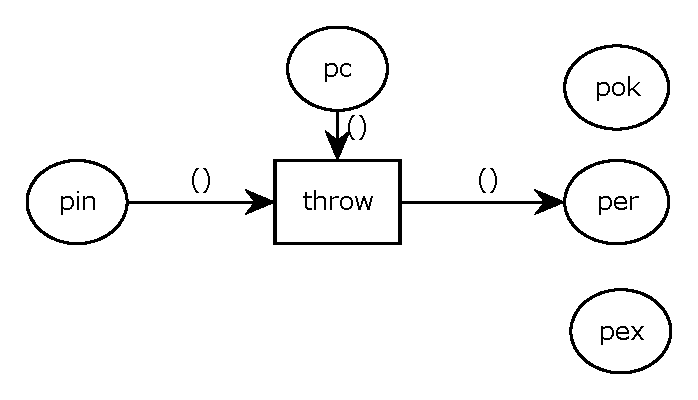
\includegraphics[scale=0.3]{Images/throw.eps}}
\hspace{0.1cm}
\subfloat[Exit PTCPN]{\label{fig:exit}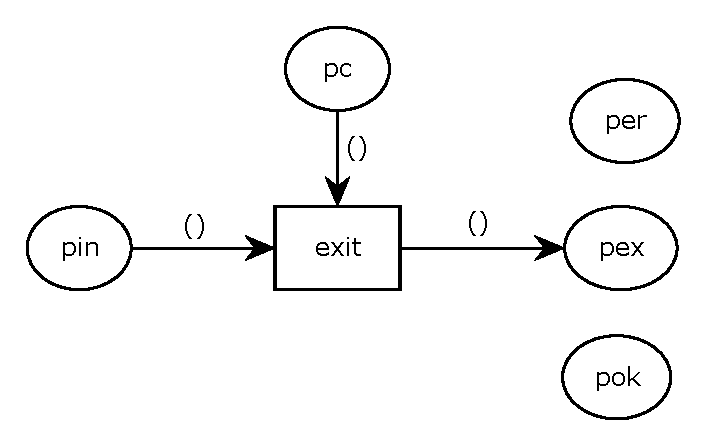
\includegraphics[scale=0.3]{Images/exit.eps}}
\hspace{0.1cm}
\subfloat[Empty PTCPN]{\label{fig:empty}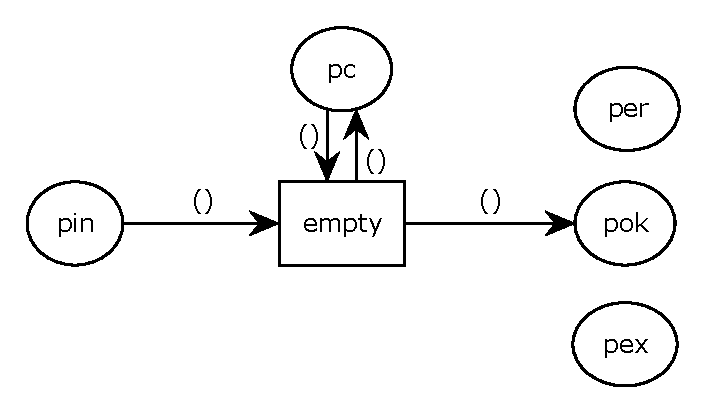
\includegraphics[scale=0.3]{Images/empty.eps}}\\
\subfloat[Wait PTCPN]{\label{fig:wait}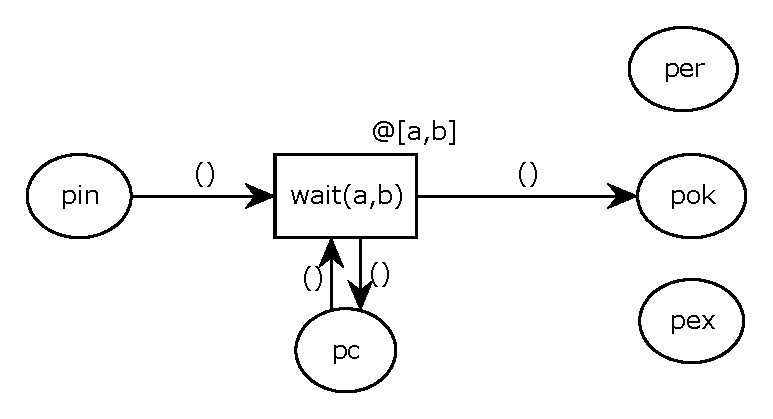
\includegraphics[scale=0.3]{Images/wait.eps}}
\ \ \ \ \subfloat[Assign PTCPN]{\label{fig:assign}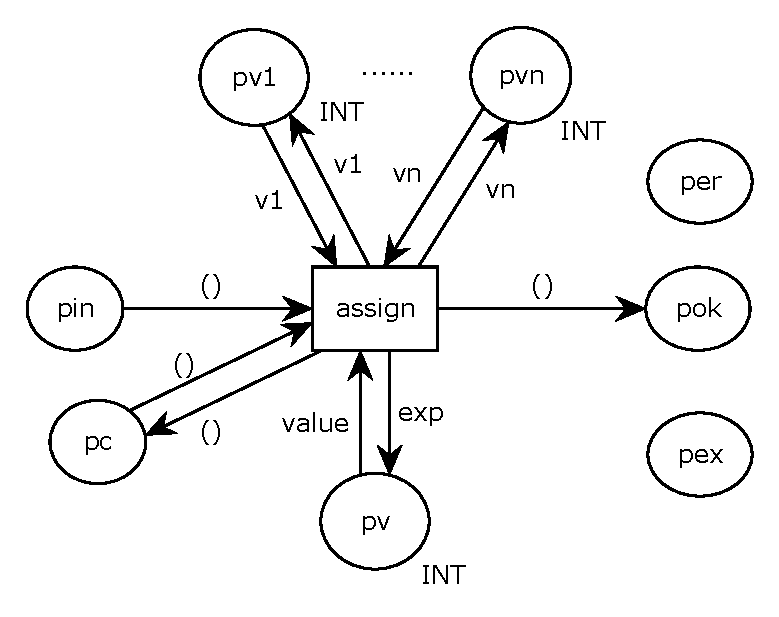
\includegraphics[scale=0.3]{Images/assign.eps}}
}}
\end{center}
\vspace{-0.5cm}
\caption{\label{fig:basicas}Basic Activities
Translation}
\vspace{-0.3cm}
\end{figure}
%\newpage

\item {\it Communication activities}:
The model we use is based on the invoke and receive operations, 
as well as the reply activity that uses a server to reply to a client. We have also added a barred version
of reply to synchronise with the response from the server. We have therefore introduced 
this last activity in our semantics to deal with the synchronous or asynchronous nature of the invoke activity (one-way or request-response operation, respectively), so the $\overline{reply}$ activity is optional in the syntax depicted in Table \ref{BPELsyntax}. 
%\vspace{-0.7cm}
\begin{figure}[!ht]
%\vspace{-0.5cm}
\hspace*{1.0cm}
\begin{center}
\fbox{ \parbox[t]{9cm}{ \center 
\subfloat[Invoke/Receive PTCPN]{\label{fig:comm1}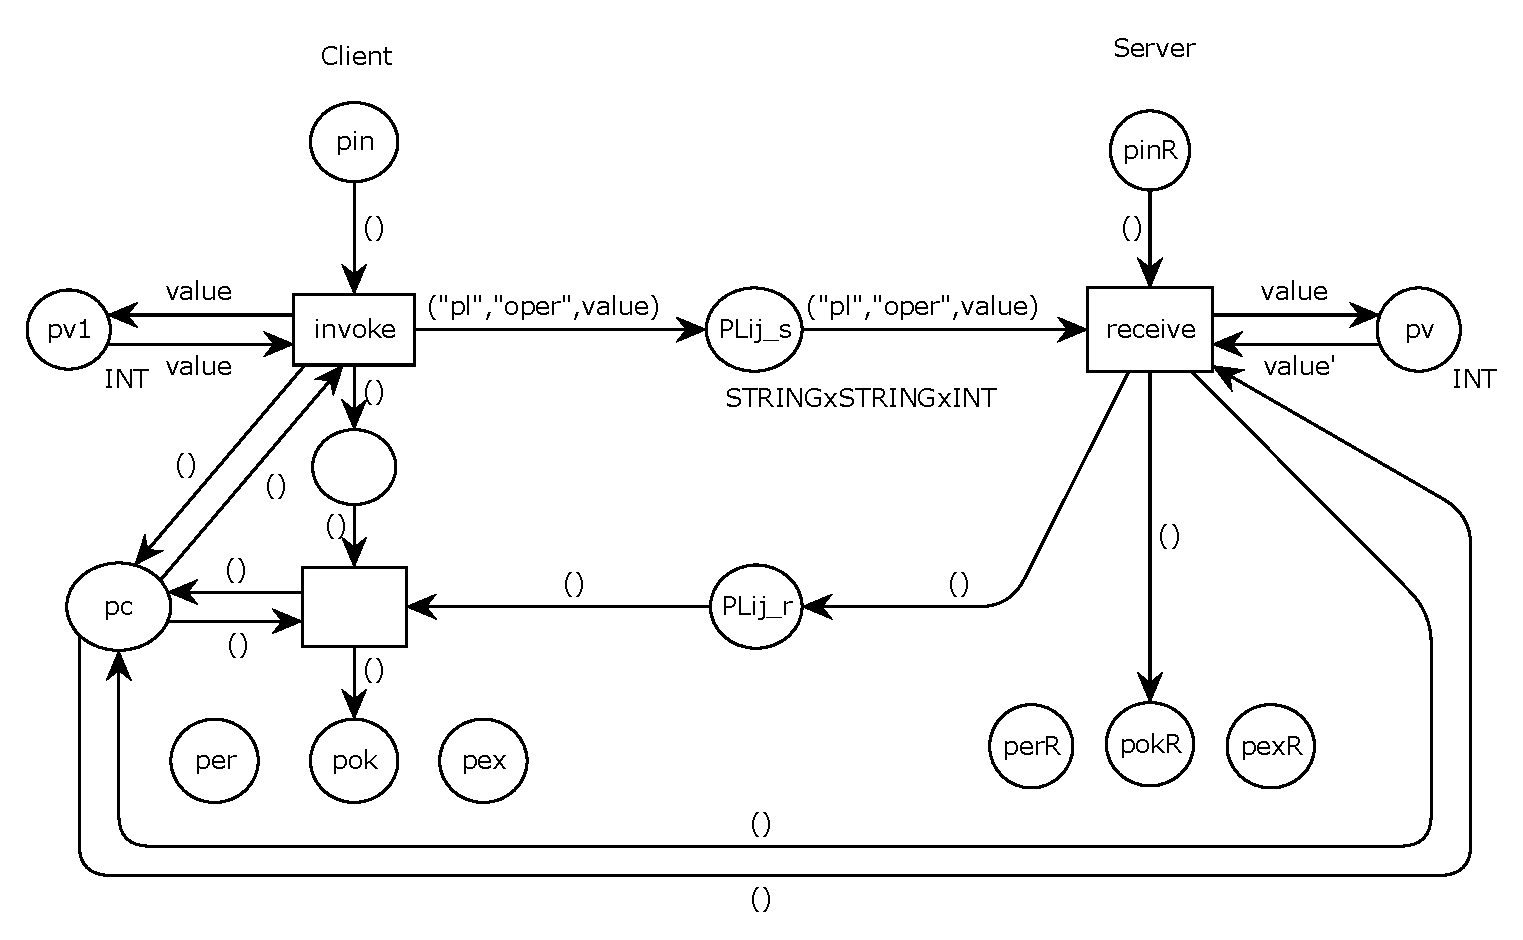
\includegraphics[scale=0.27]{Images/communication.eps}}\\
\subfloat[Reply/$\overline{Reply}$ PTCPN]{\label{fig:comm2}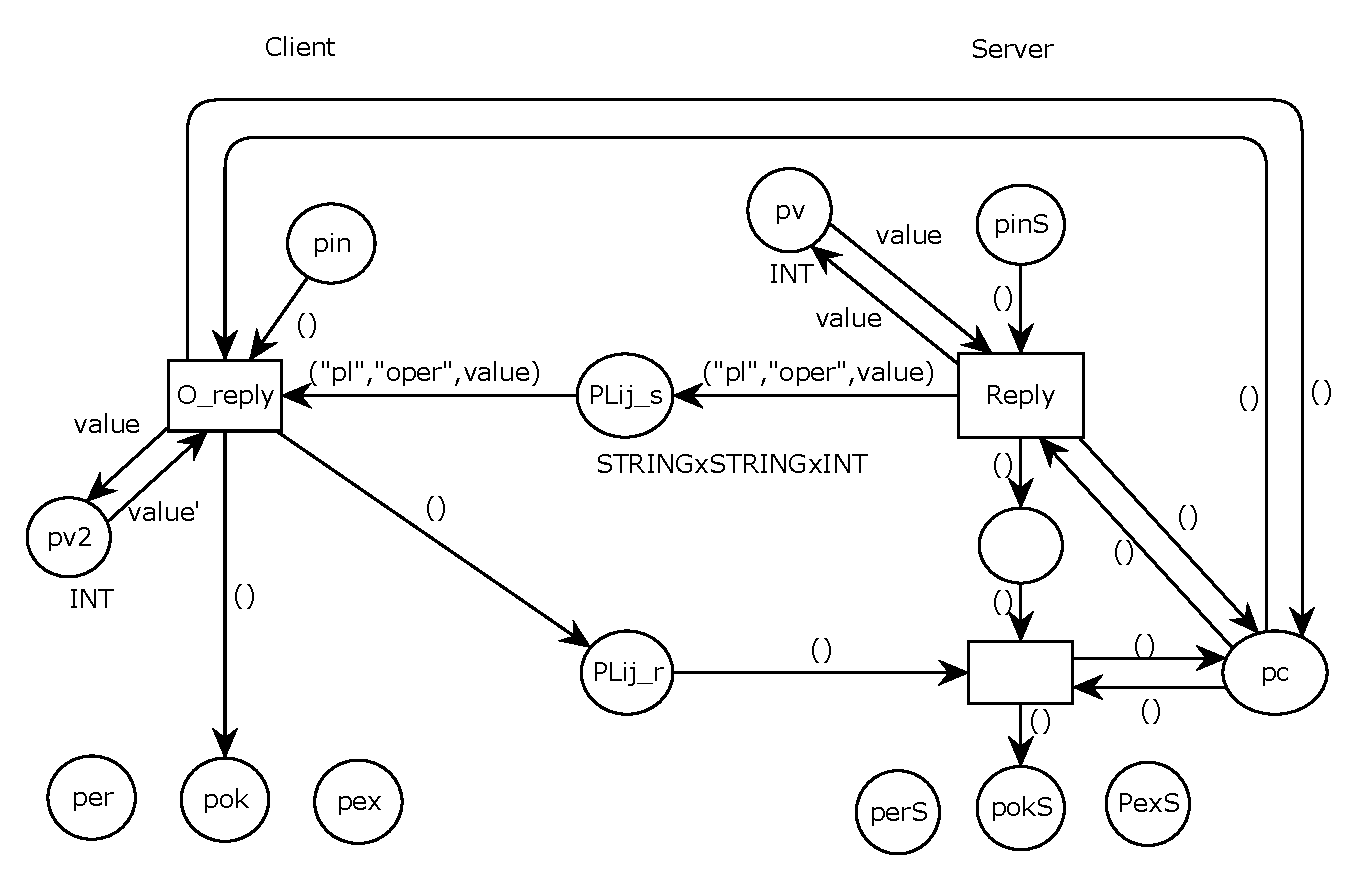
\includegraphics[scale=0.27]{Images/communication_2.eps}}
}}
\end{center}
\vspace{-0.5cm}
\caption{\label{fig:comm}Invoke/Receive Activities
Translation}% \vspace{1cm}
%\vspace{-0.5cm}
\end{figure}

%In this case, we have added to our timed Petri net two specific places in order to manage the execution of invoke/receive and reply/$\overline{reply}$, $PLij\_s$ and $PLij\_r$. Thus, we only require two places to represent all the partnerlinks between two services since we will bind each one with its corresponding counterpart by using the colours of the tokens. Place $PLij\_s$ receives tokens with three parameters: $pl,op$ and $value$, whereas $PLij\_r$ is marked only when the activity has received the data, so this place is marked with the value 0. For the sake of simplicity, we exchange only the value of the variables, but this could be easily extended to any kind of data. We depict the Petri nets in Fig. \ref{fig:comm} that express the communication among partners. In Fig. \ref{fig:comm1}, the \emph{invoke} activity extracts the value to send from the variable place ${\it P_v}$ and mark the ``sending'' partnerlink with a token endowed with this information. Once this place is marked, the receive transition can be fired marking $PLij\_r$ to allow the invoke activity to continue, and storing directly the data exchanged in the corresponding variable place. The interpretation of Fig. \ref{fig:comm2} is analogous.  
Fig.~\ref{fig:comm} shows the translation for both the invoke/receive and the reply/$\overline{reply}$ pairs of activities. Part \ref{fig:comm1} of the figure corresponds to the invoke/receive translation, in which the net of the invoke activity is depicted on the left-hand-side part, whereas the receive activity is depicted on the right-hand-side part. There are two shared places, $PL_{ij{_s}}$ and $PL_{ij{_r}}$, which are used to implement the synchronisation between the invocation and reception of services. Both places are associated to the partnerlink used for this communication, denoted here by $(i,j)$, where $i$ and $j$ are the orchestrator identifiers performing those activities. Notice that the value of a single variable is transmitted, which is obtained from the corresponding variable place, $p_v$. In the same way, the receive activity stores this value in its own variable. The interpretation of Fig.~\ref{fig:comm2} is analogous.  
\end{itemize}
%
% ======================================================================
%                            ORDERING 
%=======================================================================
\subsection{Ordering structures}

%Structured activities prescribe the order in which a collection of activities is executed. They 
%describe how a business process is created; by composing the basic activities and the WSRF-compliant activities (presented previously)
%it performs into structures that express the control patterns, handling of 
%faults and external events, and coordination of message exchanges between process instances 
%involved in a business protocol.  
WS-BPEL defines structured activities for various control-flow patterns:
\begin{itemize} 
\item Sequential control between activities is provided by $<$sequence$>$, $<$if$>$, \linebreak $<$while$>$, 
$<$repeatUntil$>$, and the serial variant of $<$forEach$>$. 
\item Concurrency and synchronization between activities is provided by $<$flow$>$ and the 
parallel variant of $<$forEach$>$.  
\item Deferred choice controlled by external and internal events is provided by $<$pick$>$.  
\end{itemize}
The set of structured activities in WS-BPEL is not intended to be minimal \cite{BPEL4WS}, so there are cases where 
the semantics of one activity can be represented using another activity. Nevertheless, in order to reduce the complexity
of our translation, our approach omits many derived activities only dealing with the most important ones from the modelling viewpoint,
such as sequence, parallel and choice. For all these cases we provide the translation
by only considering two activities. However, the generalization
to a greater number of activities is straightforward in all
of them. 
\begin{itemize}

\item {\it Sequence}\,: A sequence of two activities $A_1;A_2$ (with PTCPNs $N_{A_1}$ and
      $N_{A_2}$, respectively)
      is translated in a simple
      way (Fig.\,\ref{seq}), by just collapsing in a 
      single place (this will be
      an internal place of the new PTCPN)
      the {\it output} place $P_{ok}$ of $N_{A_1}$, and the
      {\it entry} place of $N_{A_2}$.  The {\it entry} place
      of the new PTCPN will
      be the {\it entry} place of $N_{A_1}$. The
      {\it output} place of the new PTCPN will
      be the {\it output} place of  $N_{A_2}$, and we also
      collapse the {\it exit}, {\it error} and {\it control}  places of both PTCPNs.

%\vspace{1cm}

\begin{figure}[!ht]
%\vspace{-0.5cm}
\begin{center}
\fbox{\parbox[]{6cm}{\center
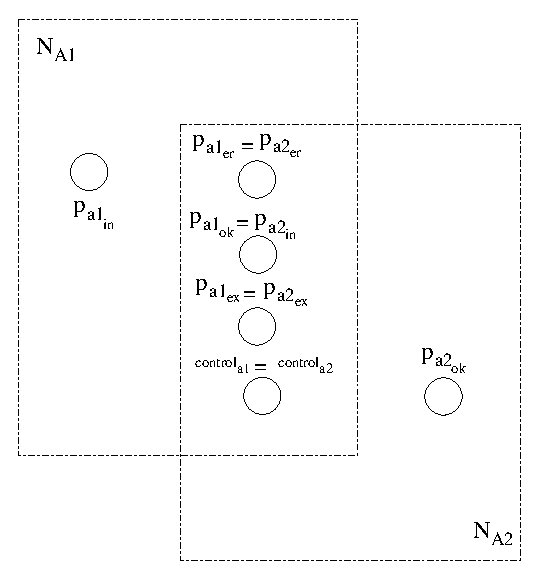
\includegraphics[scale=0.5]{Images/sequence.eps}}}
\end{center}
\vspace{-0.5cm}
\caption{\label{seq} Sequence Translation}
%\vspace{-0.6cm}
\end{figure}

\item {\it Parallel}\,: The translation for a parallel activity is depicted
in Fig.\,\ref{par}, which includes two new transitions $t1$ and
$t2$. The first to fork both parallel activities
and the second to join them when correctly terminated. 
Transition $t1$ thus puts one token on the initial places of both
PTCPNs, $N_{A_1}$ and $N_{A_2}$, in order to activate them,
and also puts one token on a new place, $p_c$, which is
used to stop the execution of one branch when the other has
failed or the exit activity is explicitly executed in one of them.
This place is therefore a precondition of every 
transition in both PTCPNs, and it is also a postcondition
of the non-failing transitions. However, in the event
of a failure or an exit activity, the corresponding {\em throw} or {\em exit}  transition
will not put the token back on $p_c$, thus
halting the other parallel activity.

Notice also that the {\em error} places of ${N}_{A_{1}}$ and $N_{A_{2}}$
have been joined in a single error place ($p_{\it er}$),
which becomes marked with one token on
the firing of one {\em throw} transition. 
In this case, the other activity cannot execute any
more actions ($p_c$ is empty), so some dead tokens would
remain permanently on some places in the PTCPN.
However, these tokens cannot cause
any damage, since the control flow has been
transferred either to the fault handling activity of the PTCPN, 
once the place $p_{er}$ has become marked, or the whole system has terminated once 
the place $p_{ex}$ is marked. %A similar reasoning is done with the {\em exit} places.
%It is a need to remark we do not treat 
%some BPEL flow construction attributes such as join conditions,
%dead path elimination, etc., since is out of the scope of this paper.
\begin{figure}[!ht]
%\vspace{-0.75cm}
\begin{center}
\fbox{\parbox[t]{12cm}
{\begin{center}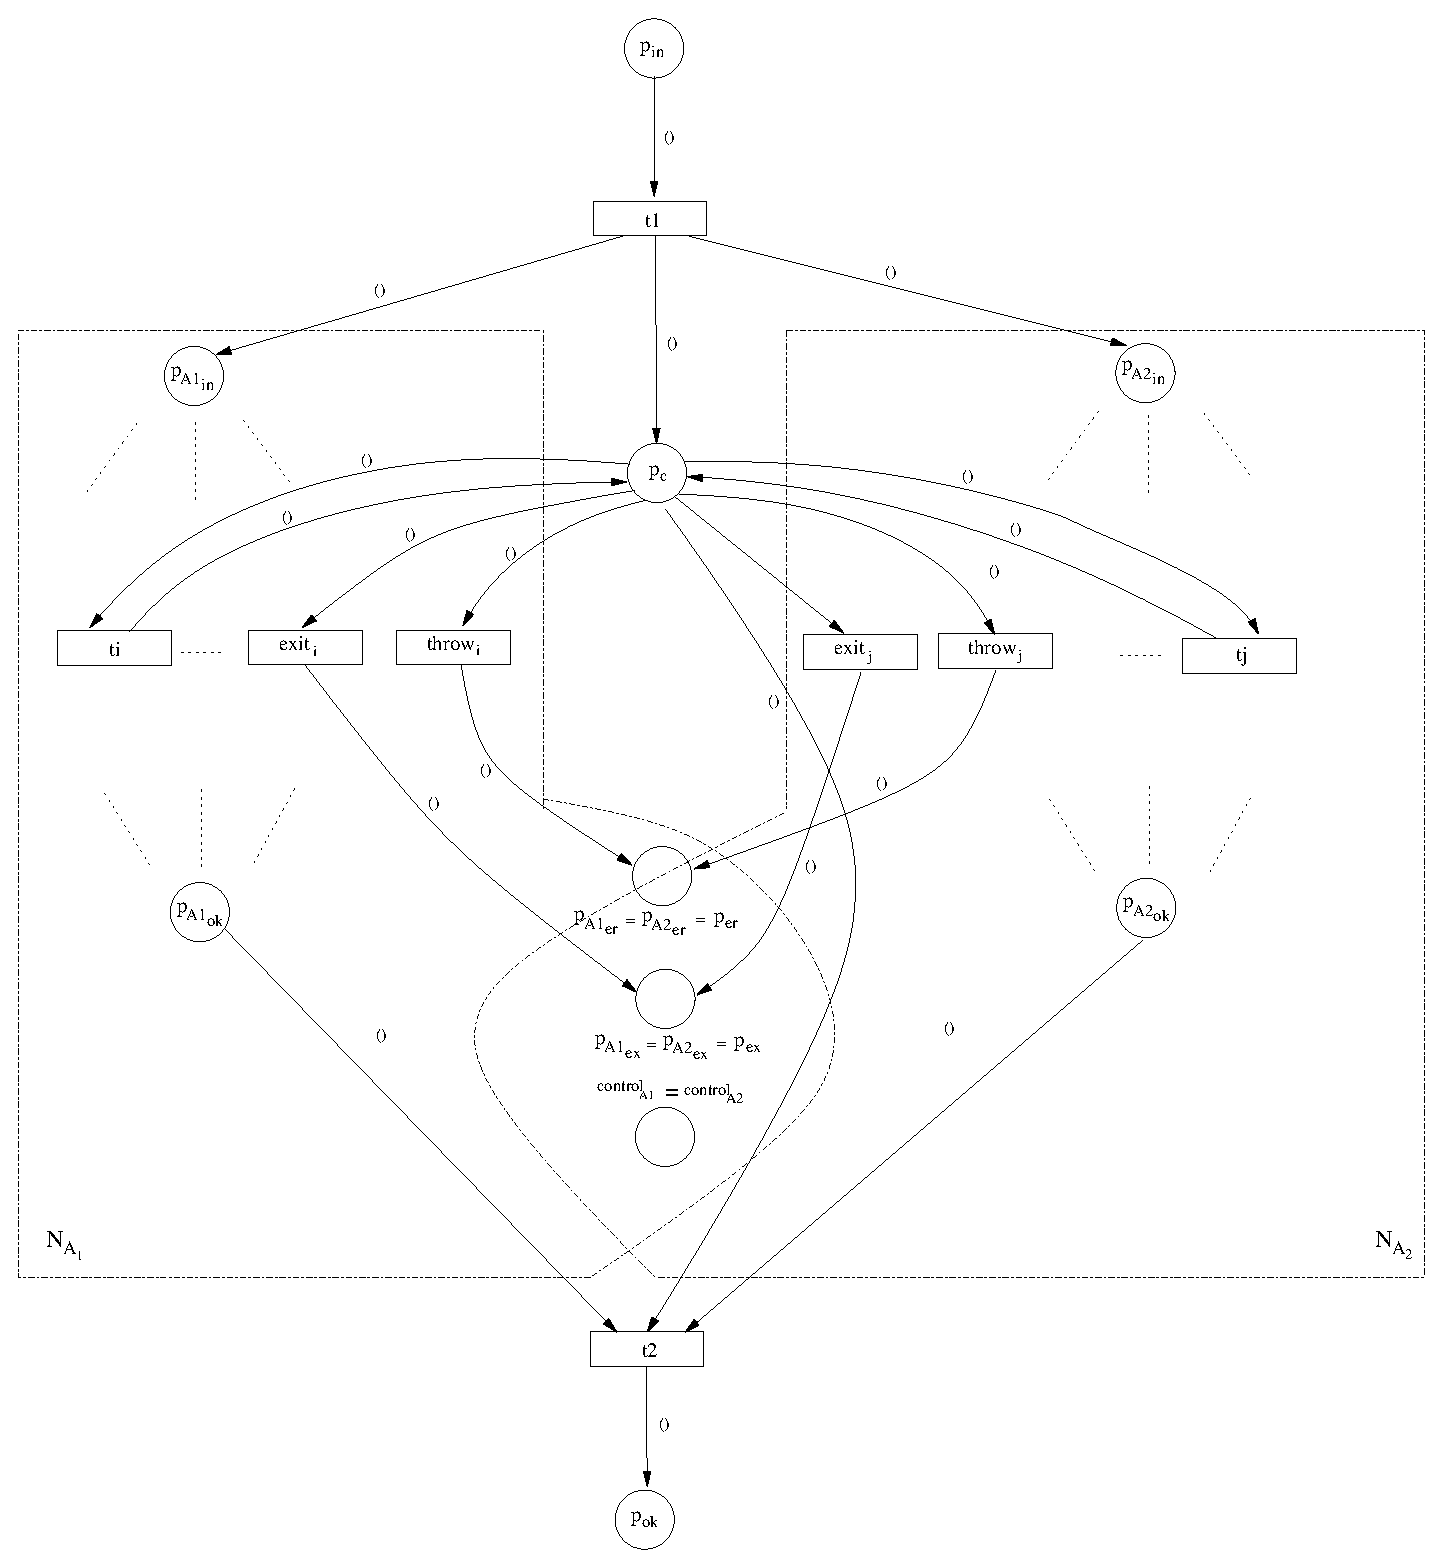
\includegraphics[height=10cm,width=12cm]
{Images/paralelo.eps}\end{center}}}
\end{center}
\vspace{-0.5cm}
\caption{\label{par} Parallel Activity Translation.}
%\vspace{-0.5cm}
\end{figure}

\item {\it Pick $(\{(pl_i,op_i,v_i,A_i)\}_{i=1}^n,A,timeout)$}: The $<$pick$>$ activity waits for the occurrence of exactly one event from a set of events, also establishing a
time-out for this selection. The translation is depicted in Fig.~\ref{pick} where a timer is implemented on the place {\it p\_a} in order to enforce the firing of transition {\it ta} when the timeout has elapsed, thus activating {\it N$_{A}$}. The colour set {\it INT} of {\it p\_a} is timed.  To illustrate how this construction works, we define the following example.
\begin{example}
In this example, there are three actors: two customers and a seller. The customers contact the
seller in order to gather information about a specific product identified by id1 and id2, respectively. The seller checks the
stock and send the requested information to the customers. The seller has established a timeout of 24 hours to receive requests. Let the orchestrations $O_{c1}=({pl_1},{id_1,id_3},A_{c1} , empty)$, $O_{c2} = ({pl_2},{id_2,id_4},A_{c2},$ $empty)$ and $O_{s} = ({pl_1,pl_2}, {id_{s1},id_{s2}, inf_{s1},inf_{s2}},A_s , empty)$ , the BPEL+ WSRFN code for the primary activity of both participants is:\\
\[\begin{array}{l}
A_{c1} = invoke(pl_1 , info, id1 ); receive(pl_1 , inforec1, id_3 ) \\
A_{c2}= invoke(pl1 , info, id1 ); receive(pl_2 , inforec2, id_4 ) \\
A_s = pick(\{(pl_1,info,id_{s1},reply(pl_1 , inforec1, id_3),(pl_2,info,id_{s2},\\
\hspace{0.9cm} reply(pl_2 , inforec2, id_4))\},empty,24)
\end{array}\]
\end{example}
\begin{figure}[!ht]
%\vspace{-0.5cm}
\begin{center}
\fbox{\parbox[c]{11.3cm}{\begin{center}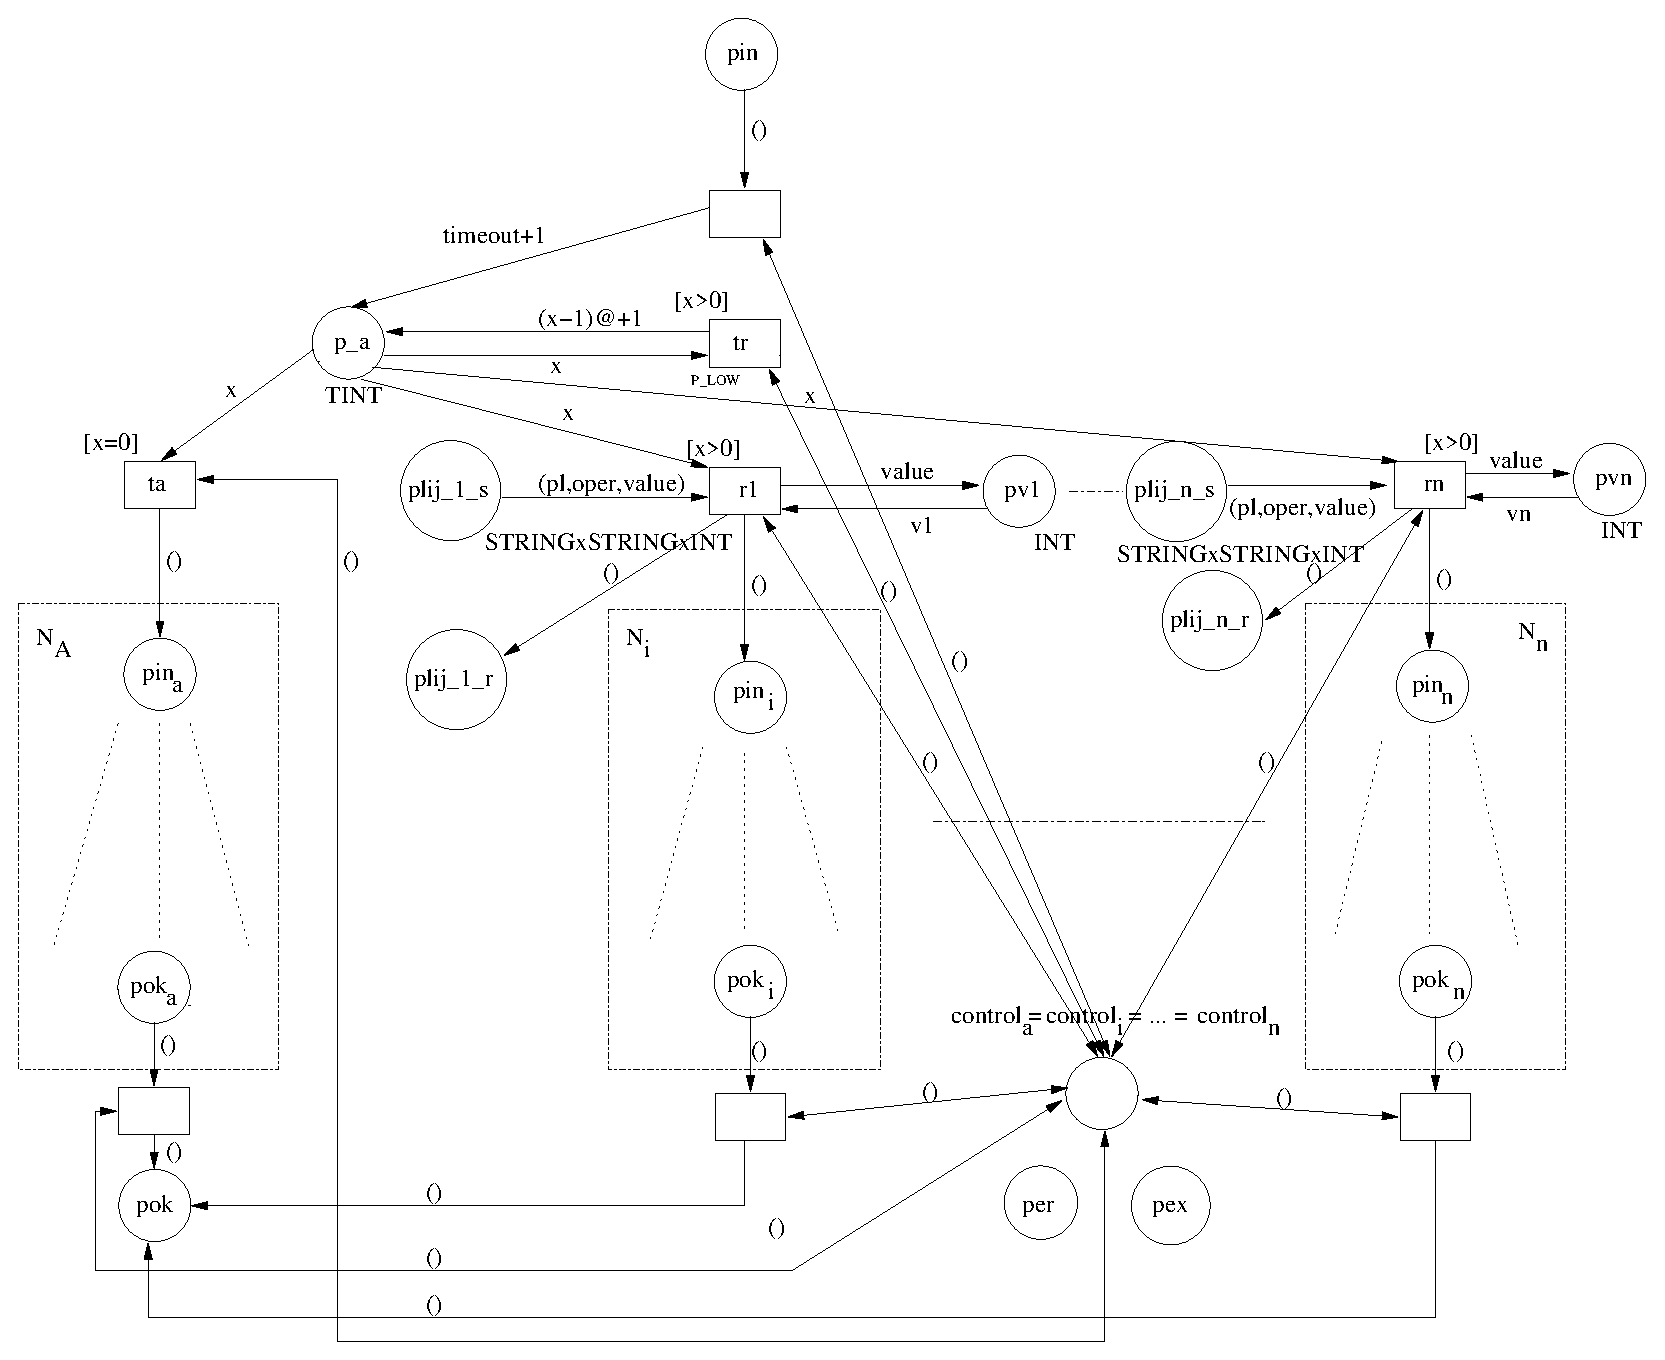
\includegraphics[scale=0.4]
{Images/pick.eps}\end{center}}}
\end{center}
\vspace{-0.5cm}
\caption{\label{pick} Pick Activity Translation.}
%\vspace{-0.4cm}
\end{figure}
Looking at Fig. \ref{pick}, it can be observed that when ${\it O_s}$ executes the \emph{pick} activity the input place ${\it p_{in}}$ of the net is marked. Next, transition ${\it t_{in}}$ is fired in order to mark the place ${\it p_a}$ with the value $timeout+1$. Two situations can then occur. One of the buyers may perform its {\emph invoke} activity before the timeout expiration, putting a token in the corresponding input place, ${\it plij_{i{_s}}}$ of the transition ${\it r_i}$, $i \in {1,..,n}$, and, then, the behaviour hereafter is the same as in the {\it receive} activity (Fig. \ref{fig:comm}). On the other hand, if none of the buyers executes an \emph{invoke} activity, the current time is increased by firing the transition ${\it t_r}$. This transition is enabled until the timeout is reached, that is, the value of $x$ is equal to 0. In that case, the PTCPN corresponding to activity $A$ is performed. We have used variable $x$ as a countdown timer due to a restriction of CPNTools, which does not allow to include the \emph{time} function in guards since its inclusion could pose side-effects\cite{CPNTools}.  
%The time delay inscription of the arc from ${\it t_r}$ to ${\it p_a}$ is necessary since CPNTools only evaluates 
%The $<$pick$>$ activity completes when the selected activity finishes.
%, then 
%executes the activity associated with that event. After an event has been selected, the other events 
%are no longer accepted by that $<$pick$>$. The $<$pick$>$ activity is comprised of a set of branches, each containing an event-activity pair.  
 %The activities contained in this construction can come in two forms: 

%\begin{itemize}
%\item The $<$onMessage$>$ is similar to a $<$receive$>$ activity, in that it waits for the receipt of an 
%inbound message. 
%\item The $<$onAlarm$>$ corresponds to a timer-based alarm. If the specified duration value 
%is zero or negative, or a specified deadline has already been reached or 
%passed, then the $<$onAlarm$>$ event activity is executed immediately. 
%\end{itemize} 
% must act in a similar fashion, but adding a feature
%which permits the selection among some activities. This selection is easy to model with Petri nets since collapsing the input places of the possible branches
%it is impossible to execute more than one at the same {\em pick}. In our model, the place {\em PinA1..An} represents this behaviour. Finally, in the BPEL specification, 
%is encouraged the use of time-outs with {\em pick} activity, so we have included a timed transition with its corresponding timed guard in order to manage the execution of 
%an ``alarm activity'' only in the event the time-out expires. The meaning of the other places and transitions is the same as in the receive activity.  

\item {\it While(cond,A)}: The machinery needed to model this construction is fairly straightforward since we only must check if the repetition condition holds or not in order to execute the contained activity or skip it. Fig.~\ref{while} shows this translation.
\end{itemize}
%The $<$while$>$ activity provides for repeated execution of a contained activity. The contained 
%activity is executed as long as the boolean condition evaluates to true at the beginning of 
%each iteration. The meaning of the places and transitions of the net represented in Fig. \ref{while} is fairly straightforward, so, due to space limitations, we are going to omit any explanation of its elements. 
%The meaning of the places and transitions are fairly straightforward, so, due to space limitations, we are going to omit any explanation of the elements contained in this net 
%\newpage


%\vspace{-1.3cm}

\begin{figure}[!ht]
%\vspace{-0.7cm}
\begin{center}
\fbox{\parbox[t]{11.3cm}{\begin{center}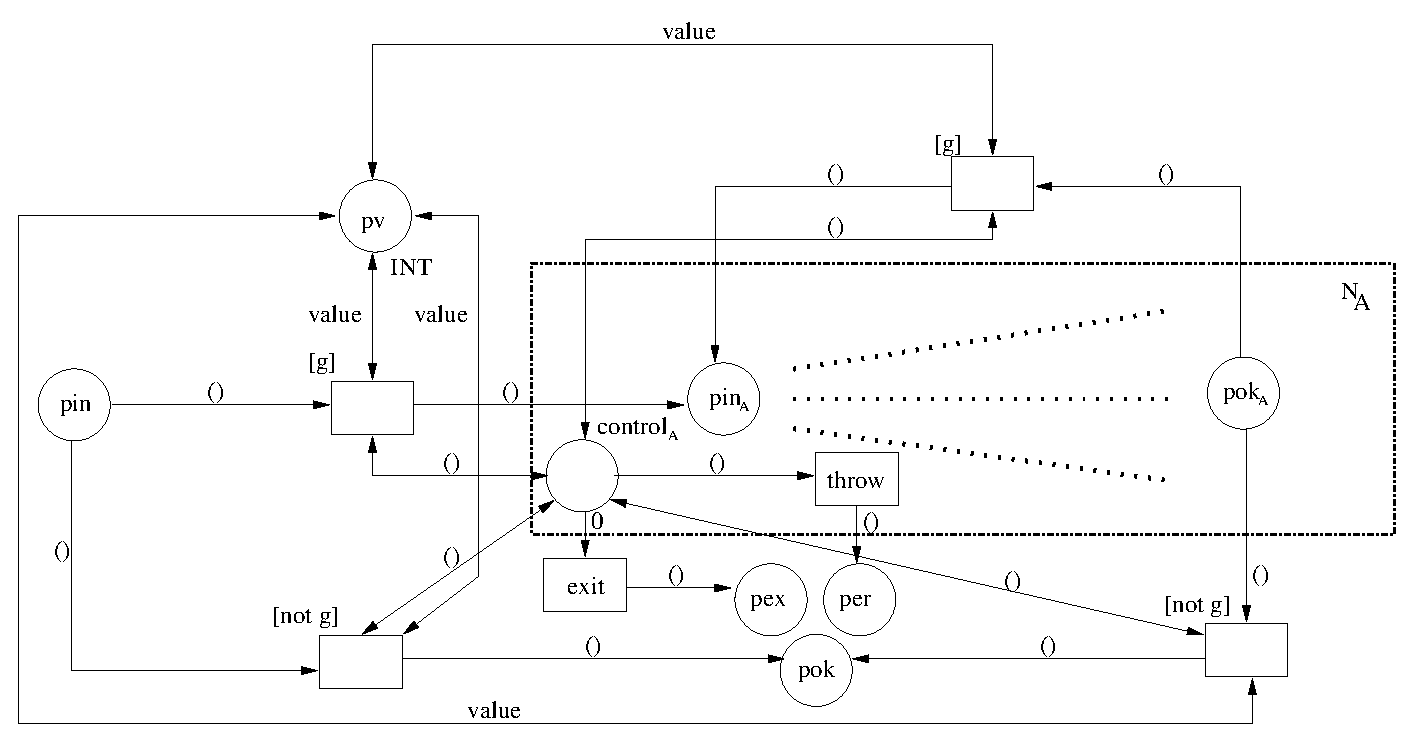
\includegraphics[scale=0.4]
{Images/while.eps}\end{center}}}
\end{center}
\vspace{-0.5cm}
\caption{\label{while} While Activity Translation.}
%\vspace{-0.7cm}
\end{figure}
\vspace{-0.5cm}
% ======================================================================
%                            WSRF 
%=======================================================================
\subsection{WSRF/WSN compliant}
%In this section, we state the WSRF activities we have integrated with the BPEL activities in order to create a framework for modelling stateful workflows. It is worth noting that in recent years have appeared a new redefinition of workflow nets which deals with resources called Resource-Constrained Workflow Nets \ref{}. As commented in the Related Work section, this approach extends the well-known formalism, Workflow nets, with finite resources such as money, memory and so on, but the authors do not provide the machinery
%to create and destroy such resources, so this extension of Workflow nets matches with the idea of WSRF standard, i.e., the creation and destruction of resources is out of the scope of the specification. Nevertheless, our approach was devised to manage the whole lifetime of the resource from its creation until its destruction.


%To date, we have presented the activities corresponding to the ``BPEL'' activities part of our model. Next, we will state the counterpart of our approach, i.e., the activities, which permit the creation and modification of the resources as well as the management of the subscriptions to them following the indications of the standard WSRF. Notice that a novelty in our model is the creation of resources since WSRF does not specify how this creation is done.
%\begin{figure}[!ht]
%\vspace{-0.5cm}
%\begin{center}
%\fbox{\parbox[t]{12cm}{\begin{center}\includegraphics[scale=0.35]
%{Images/createResource.eps}\end{center}}}
%\end{center}
%\vspace{-0.7cm}
%\caption{\label{createresource} CreateResource Activity Translation.}
%\vspace{-1.5cm}
%\end{figure}

%To begin with, we depict the creation of resources in Fig. \ref{createresource}. In order to guarantee our PTCPNs are 1-safe, we opted as commented above to model each resource with two dedicated places,  $p_{\it r_i}$, and $p_{\it r_a}$, which represent the possible state of the resources, instantiated or not instantiated, respectively. Thus, when an orchestrator wants to create a resource, the firing of the transition {\it createResource} moves the token from the ``inactive'' ($p_{\it r_i}$) to the ``active'' place ($p_{\it r_a}$) making available this resource to the subscribers. Once the place $p_{\it r_a}$ is marked and an orchestrator executes the activity {\em subscribe}, our translation can automatically build the subscriptions nets. Here, a subscription net is formed by a transition, whose guard is the subscription condition, and the subnet which corresponds to the translation of the activity that the subscriber wants to be executed just in case the subscription condition ${\it gc_i}$ holds. Notice that WSRF allows the creation of multiple subscriptions to the same resources by the same orchestrator, so we will allow this restriction. Despite the {\em subscribe} construction will be presented later, just comment here we have endowed each resource with a list that represents its subscribers with their {\em id} and an integer, $0$ or $1$, to denote whether the orchestrator with identifier {\em id} is subscribed or not. Finally, in the leftmost part of Fig. \ref{createresource}, we depict the net that will be fired in the event of the resource lifetime expires. In this situation, we return the token from the active place to the inactive place and immediately execute the activity {\em $Activity_timeisup$}, which will be passed as an argument of the {\em createResource} activity. This argument is not included in the WSRF specification, but we have incorporated it to show the benefits of the integration of both standards.       

%Now, we describe the PTCPNs who corresponds to the manipulation of resource value and lifetime as well the subscription to a specific resource. On the left side of Fig. \ref{fig:getproperty},
%the PTCPN for the activity {\em getProperty} is depicted. Here, the resource {\em value} obtained from $p_{\it r_a}$ is stored in the place of the corresponding variable. The reasoning done in the construction of the PTCPNs for the activities {\em setProperty} and {\em setTimeout} in Fig. \ref{fig:setproperty} is quite similar, but updating the resource value or its lifetime, respectively. Important to note that if an orchestrator is trying to access to a resource not instantiated, the fault place  $p_{\it er}$ will be marked starting the execution of the fault activity. 
%\begin{figure}[!ht]
%\vspace{-0.5cm}
%\hspace*{1.0cm}
%\begin{center}
%\fbox{ \parbox[t]{12cm}{ \center
%  \subfloat[GetProperty and Subscribe Activities]{\label{fig:getproperty}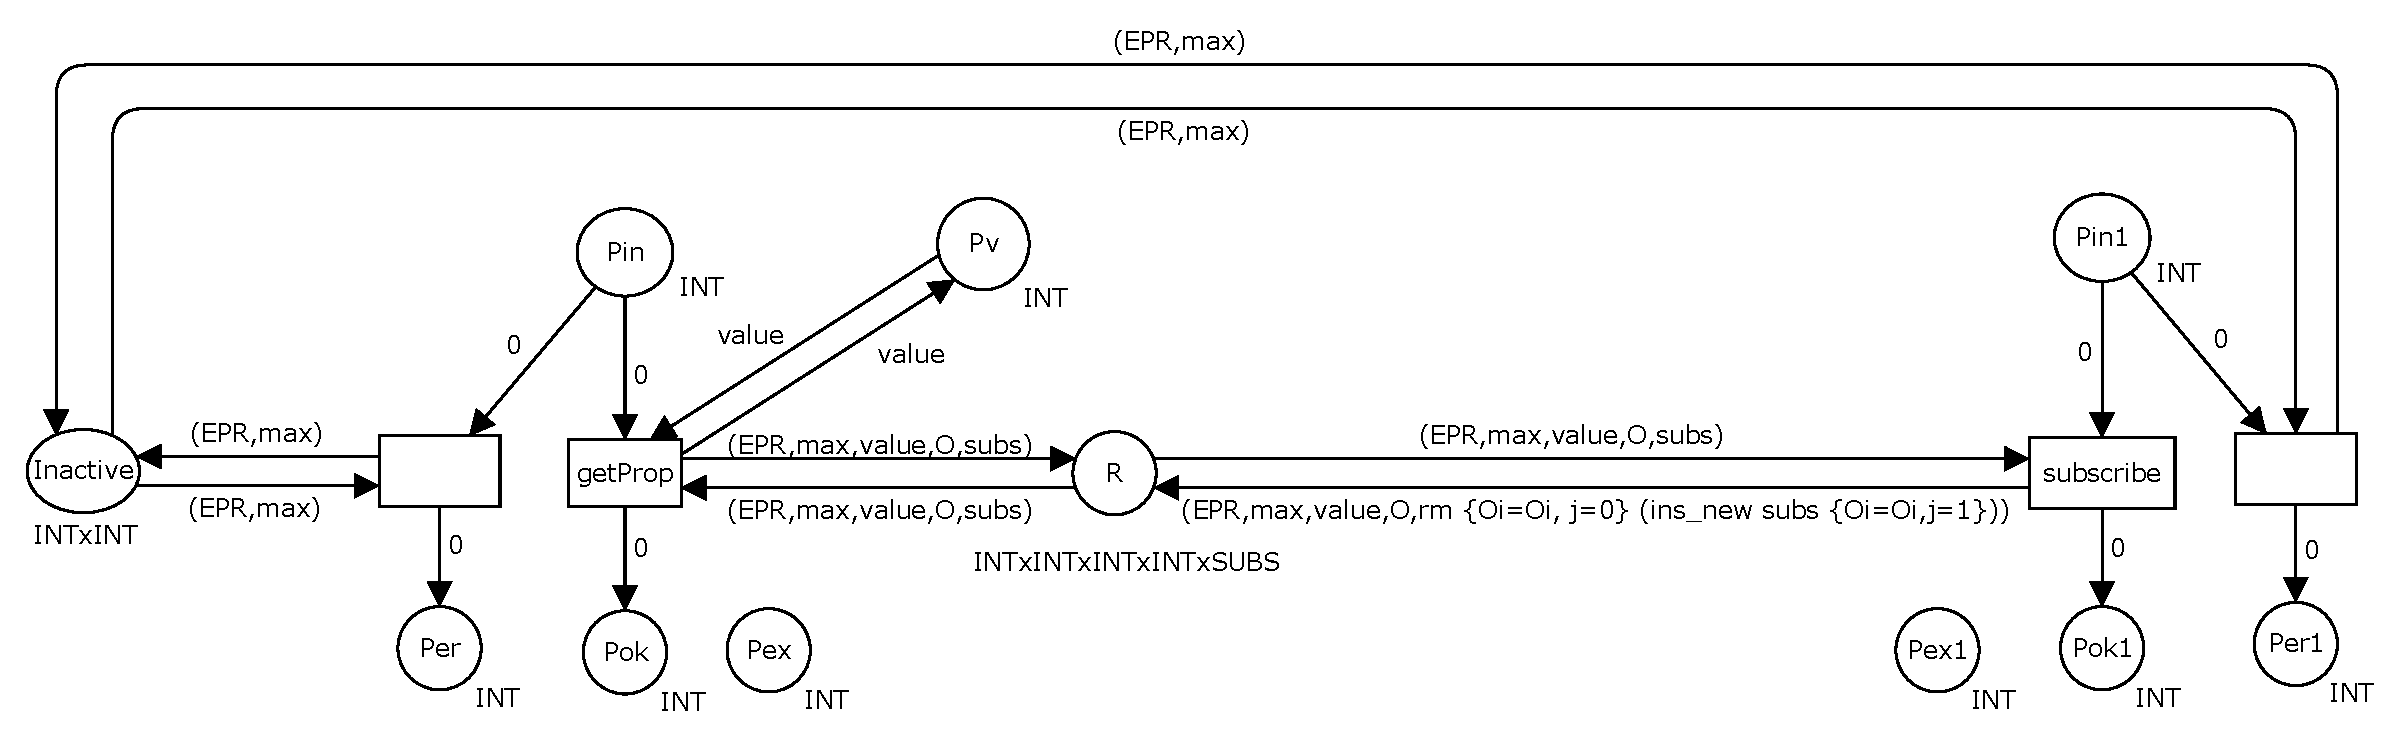
\includegraphics[scale=0.3]{Images/getProp+subscribe.eps}}\\
 % \subfloat[SetProperty and SetTimeout Activities]{\label{fig:setproperty}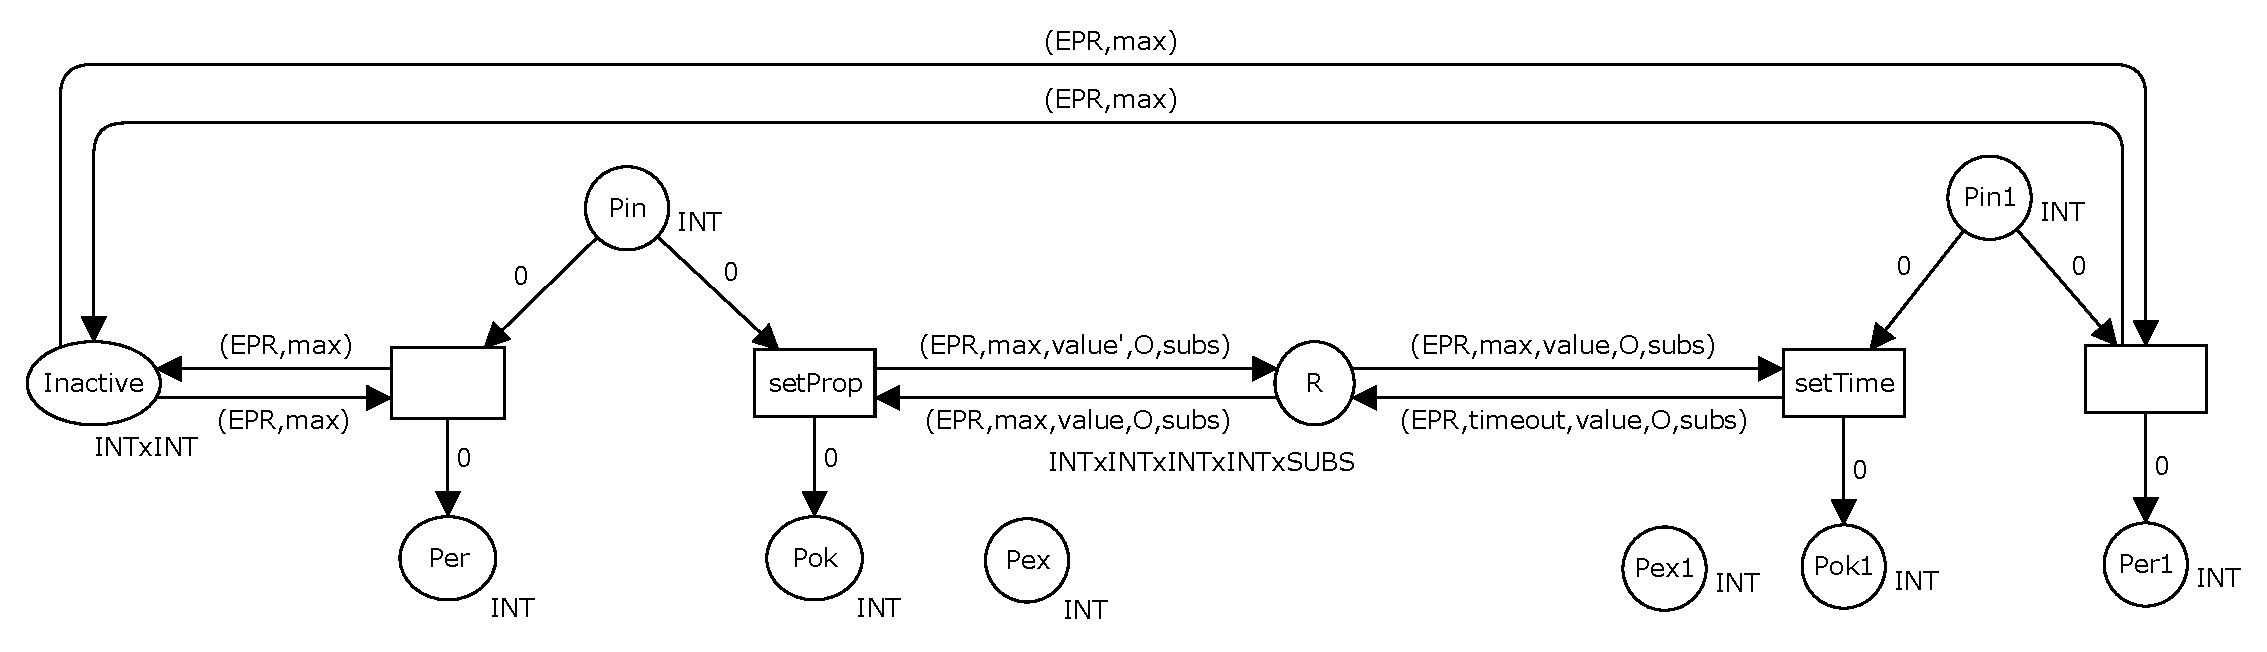
\includegraphics[scale=0.32]{Images/setProp+setTime.eps}}
 % }}
%\end{center}
%\vspace{-0.6cm}
%\caption{\label{fig_wsrf}WSRF Activities
%Translation}
%\vspace{-0.5cm}
%\end{figure}

%Finally, on the right side of Fig. \ref{fig:getproperty}, we show the PTCPN for the {\em subscribe} activity. Above, we have commented we have used a list to represent the subscribers of a resource. Since we have used CPNtools to build our nets, this ``registration stamp'' is modeled by using the record colour set provided by this tool. This record contains the identifier of the subscriber, {\em ID}, and integer variable {\em j}, whose value will be $0$ when the orchestrator is not subscribed and $1$ in the opposite case. This value will be checked in the guard of the first transition of the subscription net within the condition specified here in order to check if the orchestrator is subscribed and the condition holds. As in the previous cases, we run the fault activity if one orchestrator is trying to subscribe to non-instantiated resource.   

%\begin{figure}[!ht]
%\begin{center}
%\fbox{\parbox[t]{12cm}{\begin{center}\includegraphics[scale=0.35]
%{Images/setProp.eps}\end{center}}}
%\end{center}
%\vspace{-0.7cm}
%\caption{\label{setp} GetProperty Activity Translation.}
%\end{figure}

%\begin{figure}[!ht]
%\begin{center}
%\fbox{\parbox[t]{12cm}{\begin{center}\includegraphics[scale=0.35]
%{Images/getProp.eps}\end{center}}}
%\end{center}
%\vspace{-0.7cm}
%\caption{\label{setp} SetProperty Activity Translation.}
%\end{figure}

%\begin{figure}[!ht]
%\begin{center}
%\fbox{\parbox[t]{12cm}{\begin{center}\includegraphics[scale=0.35]
%{Images/setTime.eps}\end{center}}}
%\end{center}
%\vspace{-0.7cm}
%\caption{\label{settim} SetTimeout Activity Translation.}
%\end{figure}

%=============================Valent�n================================
Let us now see the WSRF/WSN activities, and their corresponding translations.

\begin{itemize}
\item {\it CreateResource(EPR,val,timeout,A)}:
{\em EPR} is the resource identifier, for which we have two complementary places in Fig.~\ref{createresource}, ${\it p_{r_i}}$ and ${\it p_{r_a}}$, where the sub-index represents the state of the resource: $i$ when it is inactive and $a$ when it is active. The initial value is $val$, and $A$ is the activity that must be executed when the time-out indicated as third parameter has elapsed.

We can see in Fig.~\ref{createresource} how the transition $createResource$ removes the token from the {\em inactive} place, and puts a new token on the active place, whose colour contains the following information: resource identifier (EPR), its lifetime (max), and its value (val). %the owner (O) and the list of subscribers (initially, empty).
\begin{figure}[!ht]
%\vspace{-0.7cm}
\begin{center}
\fbox{\parbox[t]{10cm}{\begin{center}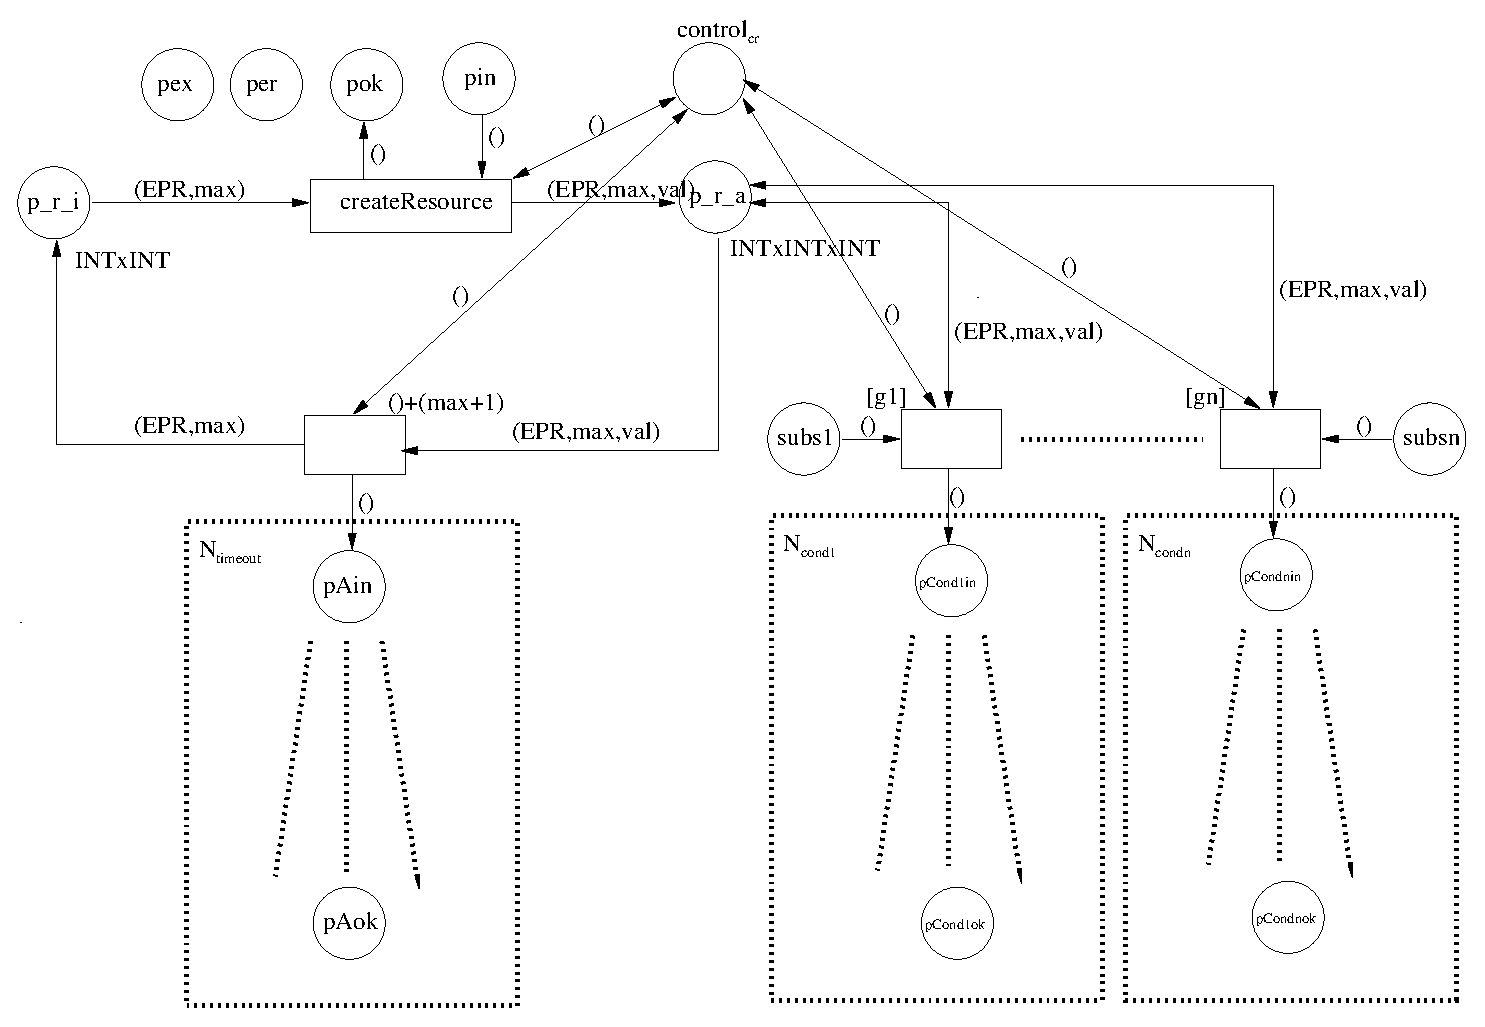
\includegraphics[scale=0.35]
{Images/createResource.eps}\end{center}}}
\end{center}
\vspace{-0.5cm}
\caption{\label{createresource} CreateResource Activity Translation.}
%\vspace{-0.5cm}
\end{figure}
Transition ${\it t}$0 is executed when the lifetime of the resource has expired, thus removing the token from the {\em active} place, marking again the {\em inactive} place, and activating $N_A$. We can also see that the {\em active} place is linked with a number of transitions, which correspond to the subscribers (we know in advance these possible subscribers from the BPEL+WSRFN document). These transitions can only become enabled if the corresponding places $subs_{i}$ are marked by performing the corresponding  activity {\em subscribe}. The PTCPNs ${\it Ncond_i}$ are the nets for the activities passed as parameter in the invocation of a subscribe activity.   
\item {\it Subscribe(EPR,cond$'$,A)}:
In this case, an orchestrator subscribes to the resource $EPR$, with the associated condition $cond'$, upon which the activity $A$ must be performed. Fig.~\ref{subscribe} shows this translation, where we can observe that the associated place $subs_{i}$ is marked in order to allow the execution of the PTCPN for the activity $A$ if the condition $g_{i}$ holds. On the contrary, if the resource is not active, we will throw the fault handling activity.
%\begin{figure}[!ht]
%\vspace{-0.5cm}
%\hspace*{1.0cm}
%\begin{center}
%\fbox{ \parbox[t]{12cm}{ \center
%  \subfloat[GetProperty and Subscribe Activities]{\label{fig:getproperty}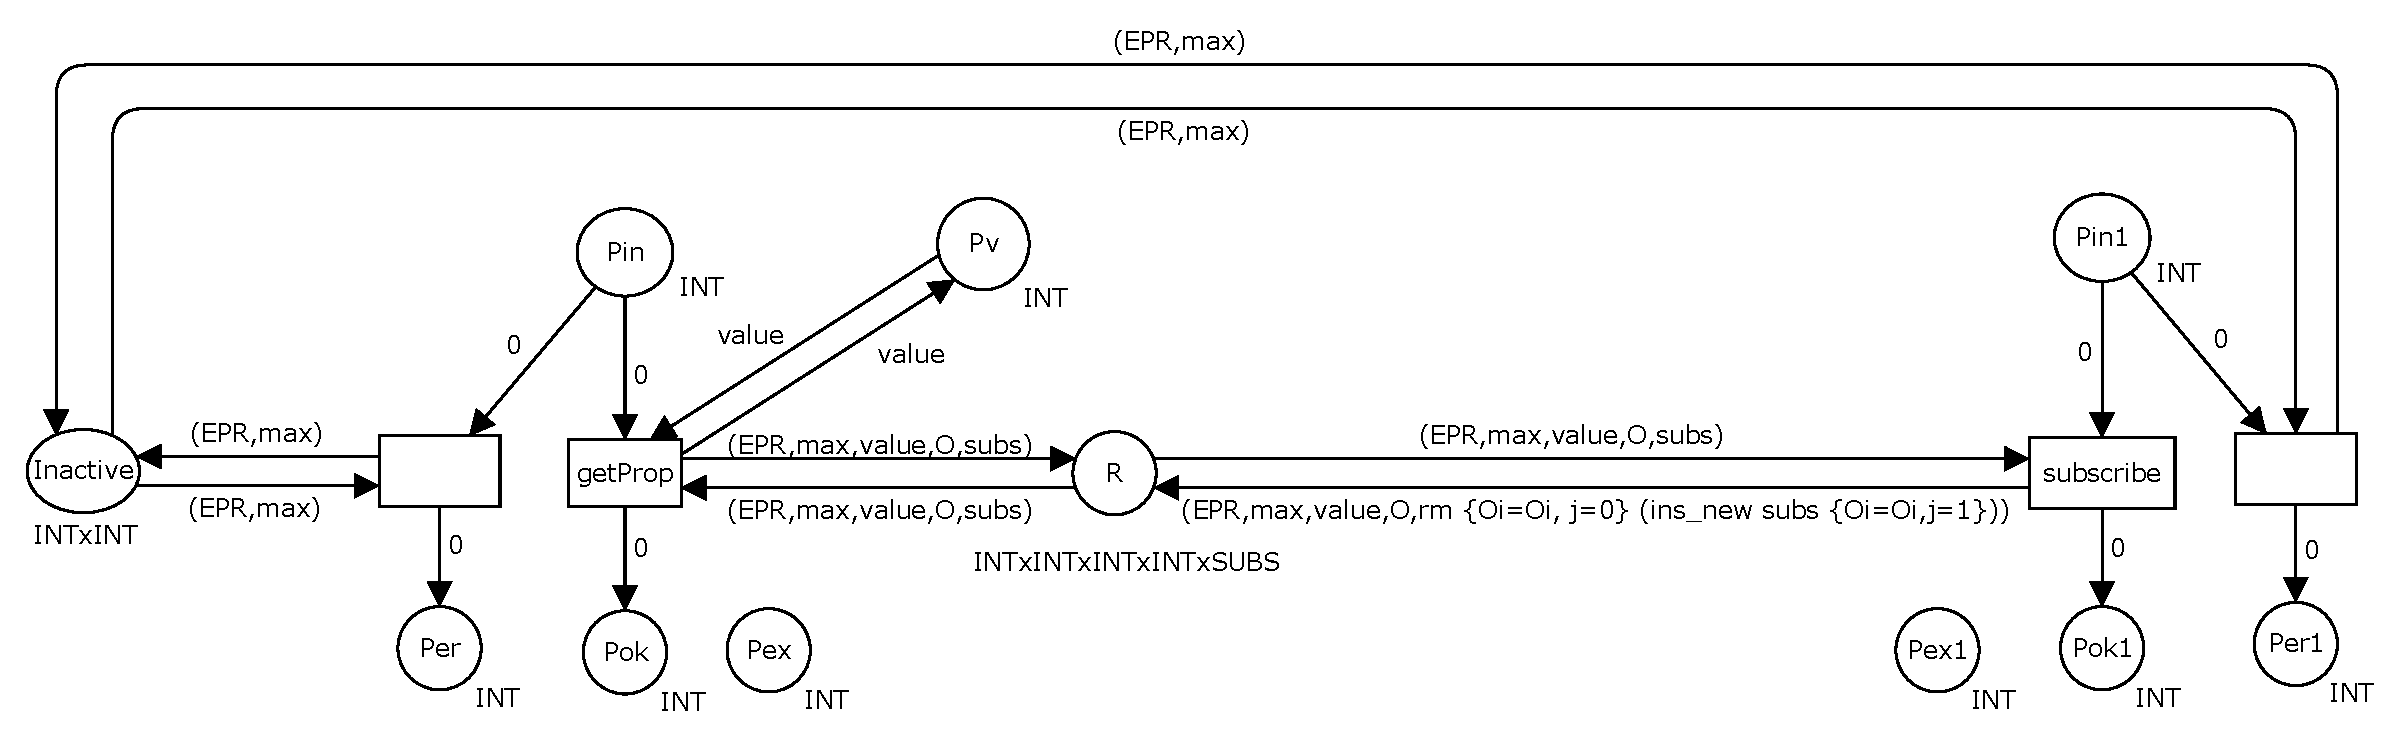
\includegraphics[scale=0.3]{Images/getProp+subscribe.eps}}\\
 % \subfloat[SetProperty and SetTimeout Activities]{\label{fig:setproperty}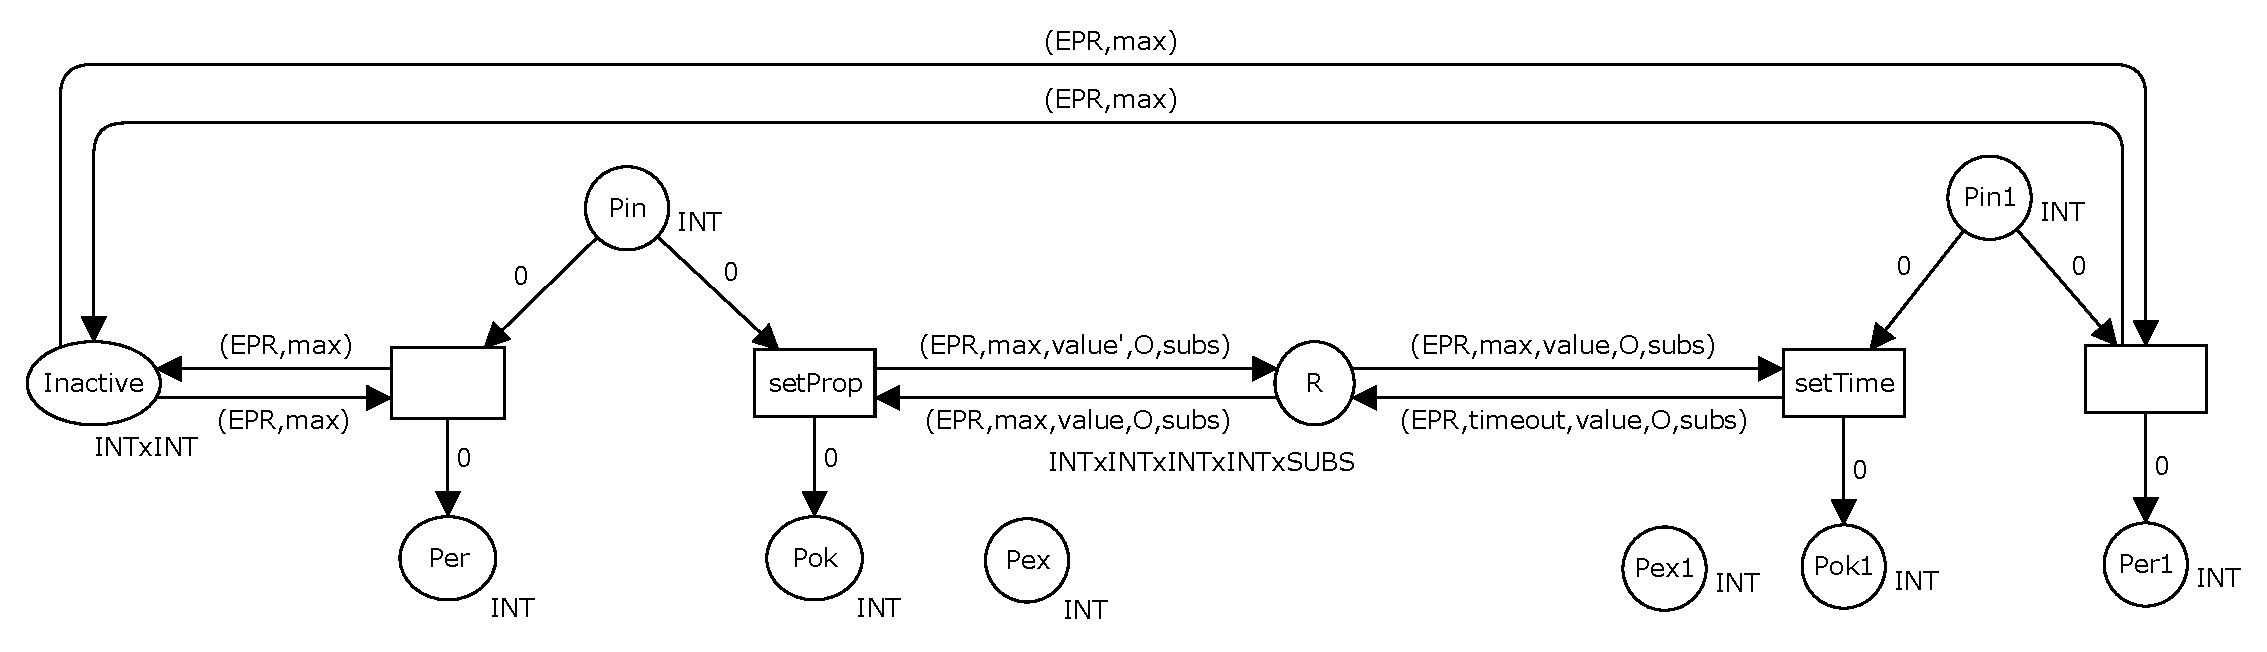
\includegraphics[scale=0.32]{Images/setProp+setTime.eps}}
 % }}
%\end{center}
%\vspace{-0.6cm}
%\caption{\label{fig_wsrf}WSRF Activities
%Translation}
%\vspace{-0.5cm}
%\end{figure}
%\newpage
\item \it{GetProp(EPR,v)} and \it{SetProp(EPR,expr)}:
These are easily translated, as shown in Figs.~\ref{getp} and \ref{setp}, where the resource value is obtained and assigned to variable $v$ (\textit{GetProp}), or a new value is assigned to the resource (\textit{SetProp}).
%\vspace{-0.8cm}

\begin{figure}[!ht]
%\vspace{1cm}
\begin{center}
\fbox{\parbox[t]{8.5cm}{\begin{center}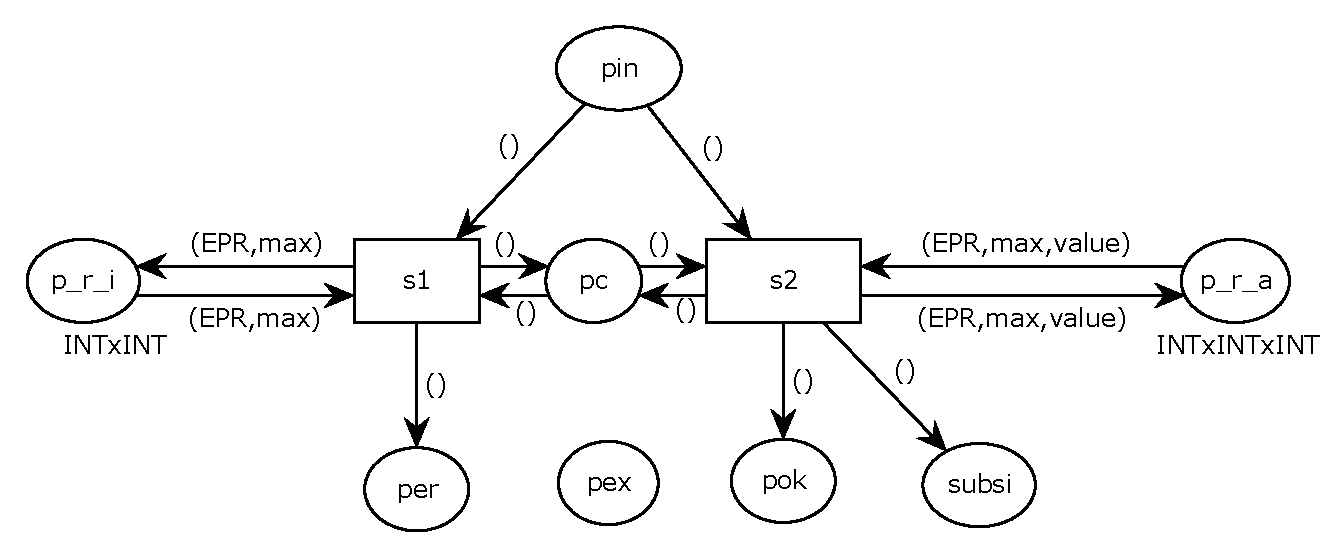
\includegraphics[scale=0.35]
{Images/subscribe.eps}\end{center}}}
\end{center}
\vspace{-0.5cm}
\caption{\label{subscribe} Subscribe Activity Translation.}
\vspace{-0.1cm}
\end{figure}

\begin{figure}[!ht]
\begin{center}
\fbox{\parbox[t]{8.5cm}{\begin{center}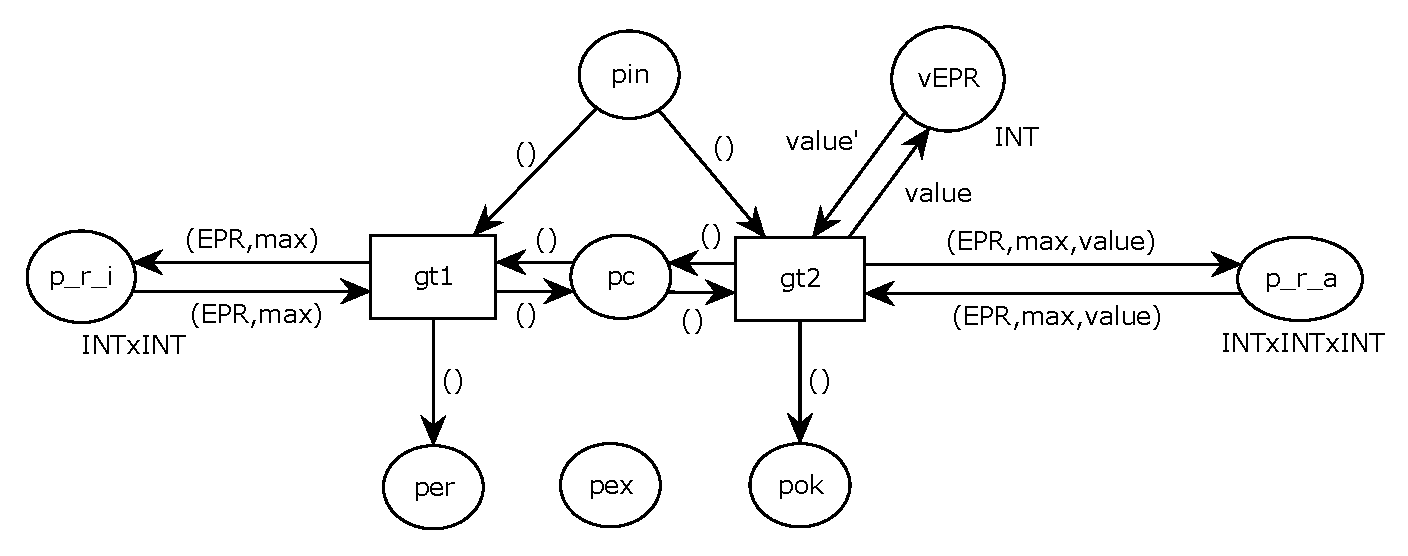
\includegraphics[scale=0.35]
{Images/getProp.eps}\end{center}}}
\end{center}
\vspace{-0.5cm}
\caption{\label{getp} GetProperty Activity Translation.}
%\vspace{-0.7cm}
\end{figure}
%\begin{figure}[!ht]
%\vspace{-0.5cm}
%\hspace*{1.0cm}
%\begin{center}
%\fbox{ \parbox[t]{11cm}{ %\center 
%\hspace{-0.2cm}\subfloat[GetProperty Activity %Translation.]{\label{fig:get}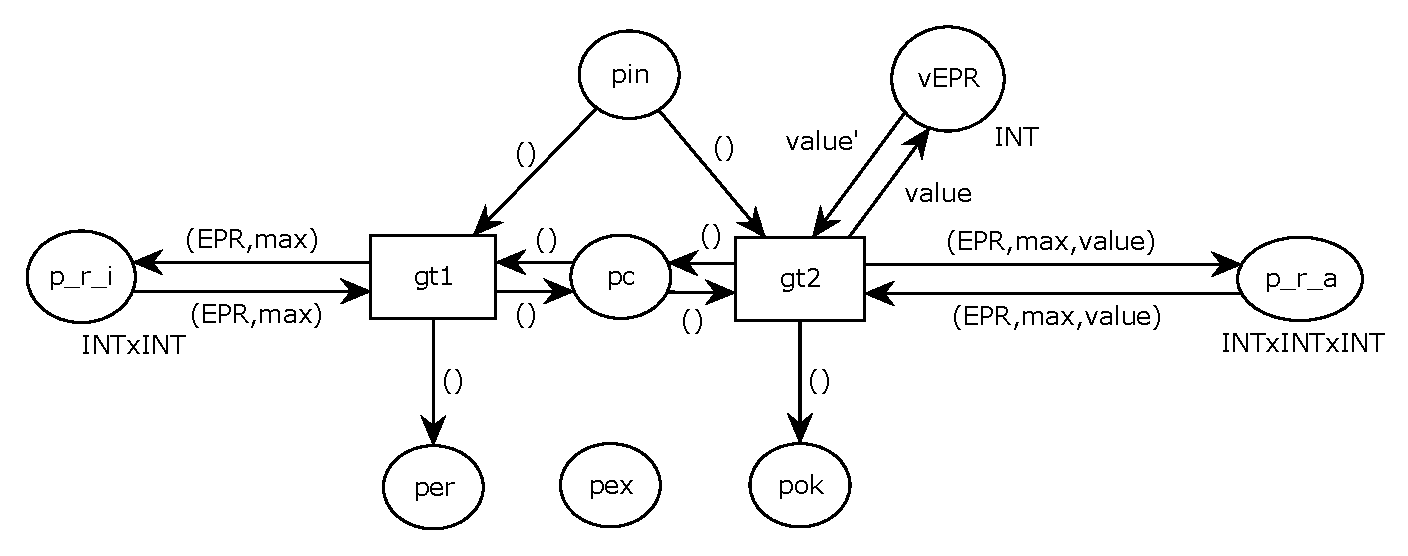
\includegraphics[scale=0.4]{Images/getProp.eps}}\\
%\subfloat[SetProperty Activity %Translation]{\label{fig:set}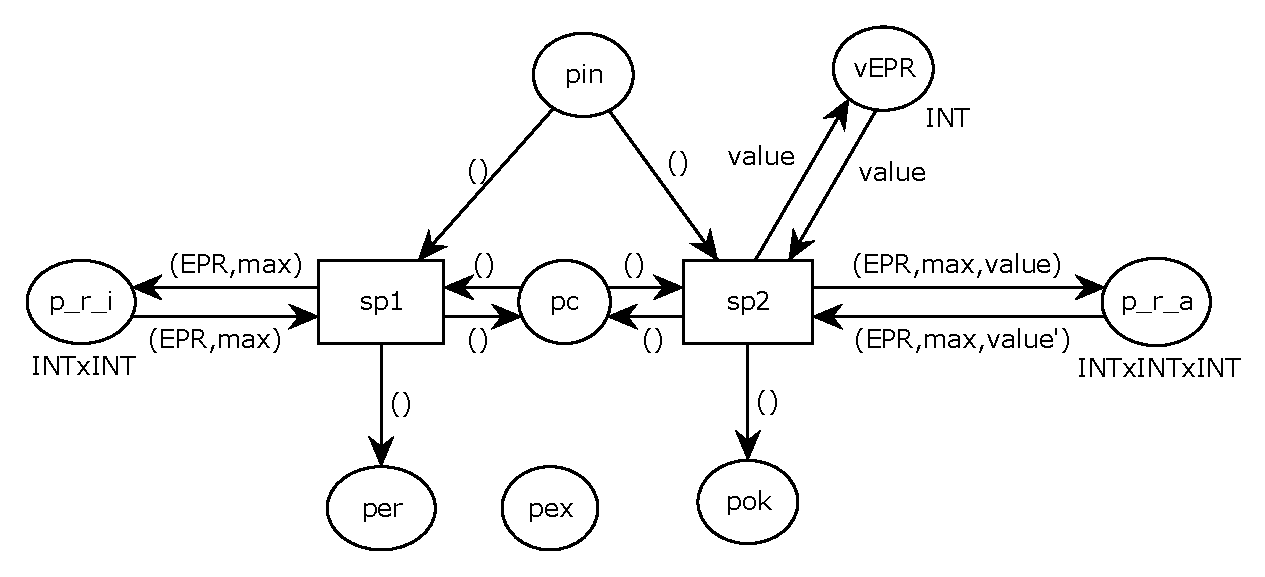
\includegraphics[scale=0.4]{Images/setProp.eps}}\\
%\subfloat[SetTimeout Activity %Translation]{\label{fig:settime}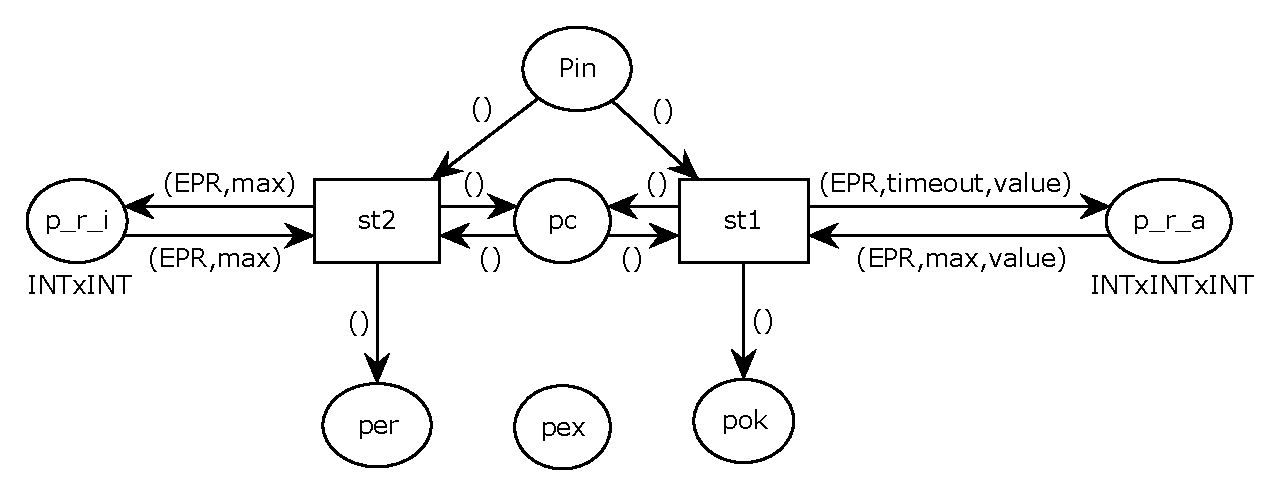
\includegraphics[scale=0.4]{Images/setTime.eps}}
%}}
%\end{center}
%\vspace{-0.62cm}
%\caption{\label{fig:sg}GetProperty and SetProperty Activities
%Translation}% \vspace{1cm}
%\vspace{-0.1cm}
%\end{figure}
%
%\newpage
\begin{figure}[!ht]
\begin{center}
\fbox{\parbox[t]{8.5cm}{\begin{center}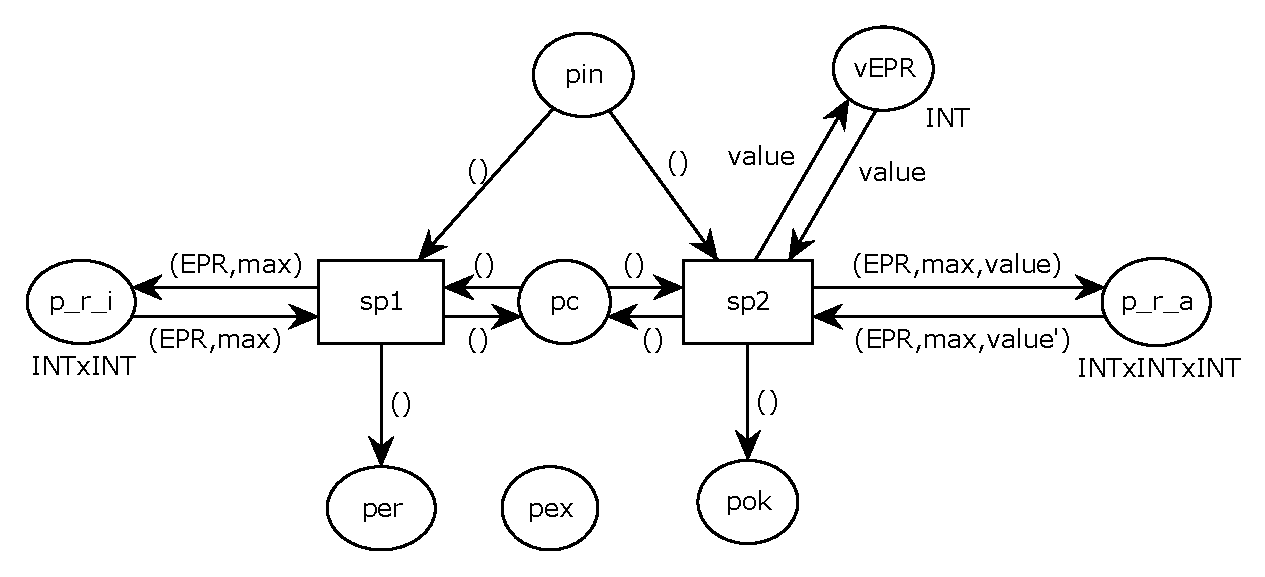
\includegraphics[scale=0.35]
{Images/setProp.eps}\end{center}}}
\end{center}
\vspace{-0.5cm}
\caption{\label{setp} SetProperty Activity Translation.}
%\vspace{0.5cm}
\end{figure}

\item {\it SetLifeTime(EPR,timeout)}:
This activity is analogous to {\em SetProp} activity. In this case, the resource lifetime is updated with a new value. Fig.~\ref{setp} shows this translation. 
\begin{figure}[!ht]
\begin{center}
%\vspace{-0.5cm}
\fbox{\parbox[t]{8.5cm}{\begin{center}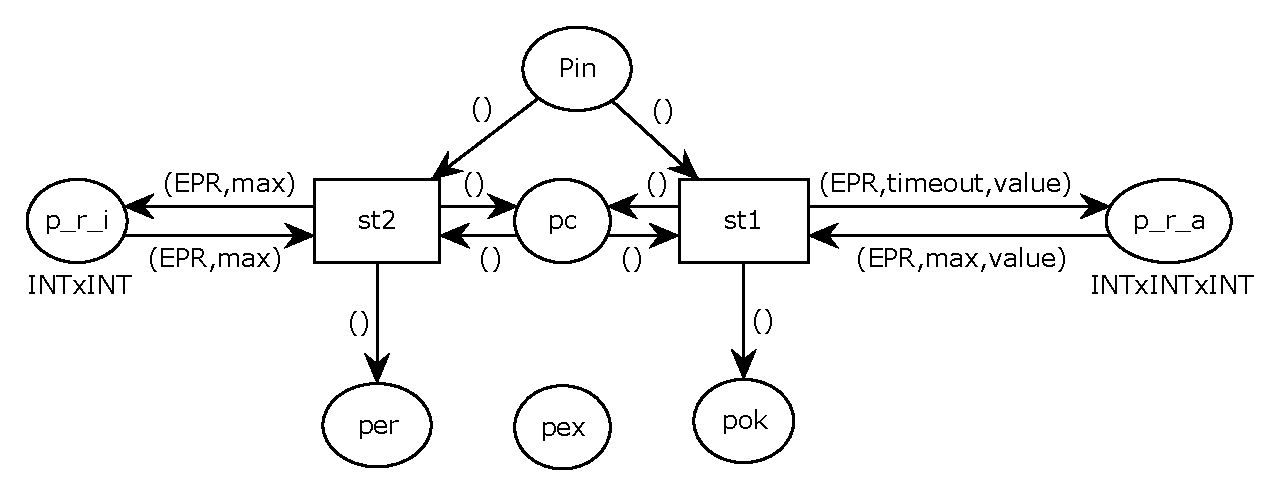
\includegraphics[scale=0.35]
{Images/setTime.eps}\end{center}}}
\end{center}
\vspace{-0.5cm}
\caption{\label{settim} SetLifeTime Activity Translation.}
%\vspace{-0.5cm}
\end{figure}
\end{itemize}

\subsection{Orchestration translation}
Once we have defined the translation for the activities, we can now introduce the definition
for the PTCPN at the orchestration level. Notice that all PTCPNs generated for
the different orchestrators cooperate to form  the entire system.

Let us call $N_A$, $N_{f}$ and $N_{e_i}$ the PTCPNs that
are obtained by applying the translation to each one of these
activities $A$, $A_f$, $A_{e_{i}},$ with $i\in\{1,m\}$:
%
\[
\begin{array}{lll}
N_A = (P_a, T_a, A_a, V_a, G_a, E_a, \lambda_a, D_a) &
\hspace*{0.6cm} & {\rm
(PTCPN~for~}A)\\
N_f = (P_f, T_f, A_f, V_f, G_f, E_f, \lambda_f, D_f)  &
\ & {\rm (PTCPN~for~}A_f)\\
N_{e_i} = (P_{e_i}, T_{e_i}, A_{e_i}, V_{e_i}, G_{e_i}, 
E_{e_i}, \lambda_{e_i}, D_{e_i})  &
\ & {\rm (PTCPN~for~}A_{e_i}\,)
\end{array}
\]

Let $p_{a_{\it in}}$, $p_{f_{\it in}}$ and $p_{{e_i}_{\it in}}$ be the initial places of
$N_A$, $N_f$ and $N_{e_i}$respectively; $p_{a_{\it ok}}$, $p_{f_{\it ok}}$ and $p_{{e_i}_{\it ok}}$ their {\em correct}\, output places, $p_{a_{\it er}},\, p_{f_{\it
er}}$ and $p_{{e_i}_{\it er}}$ their {\em error}\, places and, finally, $p_{a_{\it ex}},\, p_{f_{\it ex}}$ and $p_{{e_i}_{\it ex}}$ their {\em exit}\, places. The PTCPN for the
orchestrator is then constructed as indicated in Fig. \ref{orchestator}. This PTCPN is then activated by putting one token
$0$ on $p_{a_{\it in}}$. However, we can have other marked places, 
for instance, those associated with integer
variables or resources. The other places are initially unmarked.
%where we are joining the following places:
%
%\[\begin{array}{ l l l}
%p_{o_{\it in}} & = & p_{a_{\it in}} =  p_{{e_i}_{\it in}}\\
%
%p_{o_{\it er}} & = & p_{f_{\it ok}} = p_{f_{\it er}}\\
%
%p_{o_{\it ok}} & = & p_{a_{\it ok}} = p_{{e_i}_{\it ok}}\\
%
%p_{a_{\it er}} & = & p_{f_{\it in}}  =  p_{{e_i}_{\it er}}
%\end{array}
%\]
%
%and the remaining places, transitions and edges are the same as
%in $N_a$, $N_f$ and $N_{e_i}$.
% Marcado inicial:
%The PTCPN is then activated by putting one token
%$0$ on $p_{o_{\it in}}$. 
%
%
%as we mentioned when we introduced the PPTCPNs. 
%The other places are initially unmarked.

\begin{figure}[!ht]
%\vspace{-0.5cm}
\begin{center}
\fbox{ \parbox[t]{8cm}{ \center 
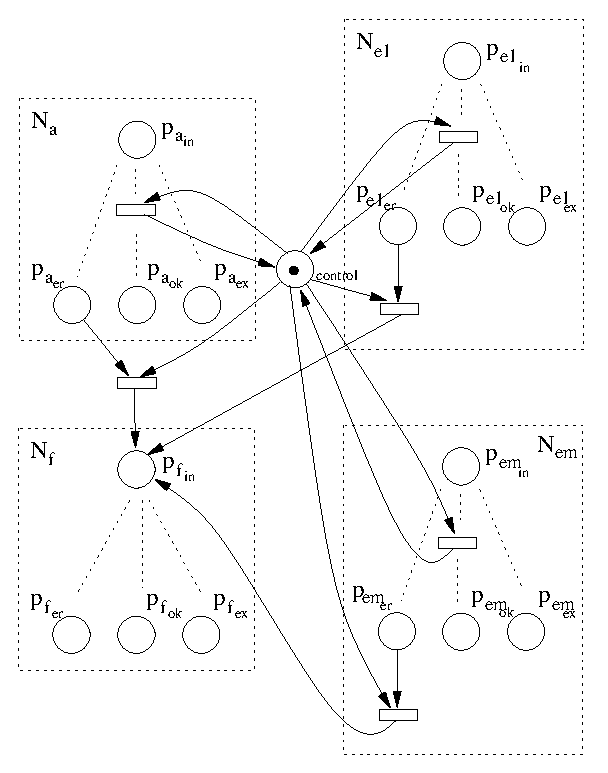
\includegraphics[scale=0.5]{Images/orchestration.eps}
}}\end{center}
\vspace{-0.5cm}
\caption{Orchestration Translation}\label{orchestator}
%\vspace{-0.5cm}
\end{figure}





%\input{ptcpn.tex}

%\input{PTCPN_mere.tex}

%\input{safeness.tex}

\section{Case Study: Automatic management system for stock market investments}\label{cs}

The case study concerns a typical automatic management system for stock market investments, which consists of {\em n+1} participants:
the online stock market system and {\em n} investors, A$_i$, $i=1,\ldots, n$. Here, the resource will be the stocks of a company that the investors want to buy just in case the price falls below an established limit, which the investors fix previously by means of subscriptions, i.e., an investor subscribes to the resource (the stocks) with a certain guard (the value of the stocks he/she want to pay for it). The lifetime {\em lft} will be determined by the stock market system and the resource price will be fluctuating to simulate the rises/drops of the stock. Notice that we do not take into account the stock buy process since our aim is to model an investors' information system. Thus, the participants will be notified when their bids hold or the resource lifetime expires.  
Let us consider the choreography ${\it C=(O_{sys},O_1,\ldots,O_n)}$, where 
\mbox{${\it O_k=(PL_k,Var_k,A_k,A_{f{_k}},\mathcal{A}_{e{_k}})}$,~k=sys,~1,...,~n;}~\mbox{${\it Var_{sys}=}$} ${\it \{at,vEPR\}, Var_i=}$ \\ ${\it  \{v_i\},\ A_{f{_k}}= exit}$. Variable $v{EPR}$ serves to temporarily store the value of the resource property before being sent; $v_i$ is the variable used for the interaction among participants, and, finally, $at$ controls the period of time in which the auction is active. Note that the value {\em x} indicates the resource value at the beginning, {\em at0} is the time that the ``auction'' is active, and, finally, {\em $x_i$} is the value of the stocks that he/she wants to pay for. We assume that all variable values are initially $0$: 
%\vspace{-0.3cm}
\begin{flushleft}
\small{ 
${\it Asys=assign(x+1,vEPR);assign(at0,at);CreateResource(EPR,lft,x,empty);}$\\
\hspace{1.1cm}${\it  while(actualTime()<=at,Abid)}$\\
${\it Abid=getProp(EPR,vEPR);assign(vEPR+bid(),vEPR);setProp(EPR,vEPR);} $ \\ \hspace{1.1cm}${\it wait(1,2)}$\\
${\it A_i=wait(1,2);subscribe(O_i,EPR,EPR<x_i,Acond_i);} $ \\ \hspace{0.8cm}${\it pick((pl_i,buy,v_i,empty),empty,at0)}$\\
${\it Acond_i=getProp(EPR,vEPR);invoke(pl_i,buy,vEPR)}$\\
}
\end{flushleft}

Here, the function {\it bid} is used to increase/decrease the stocks value simulating the fluctuation of the stocks price.

\begin{figure}[h]
\fbox{
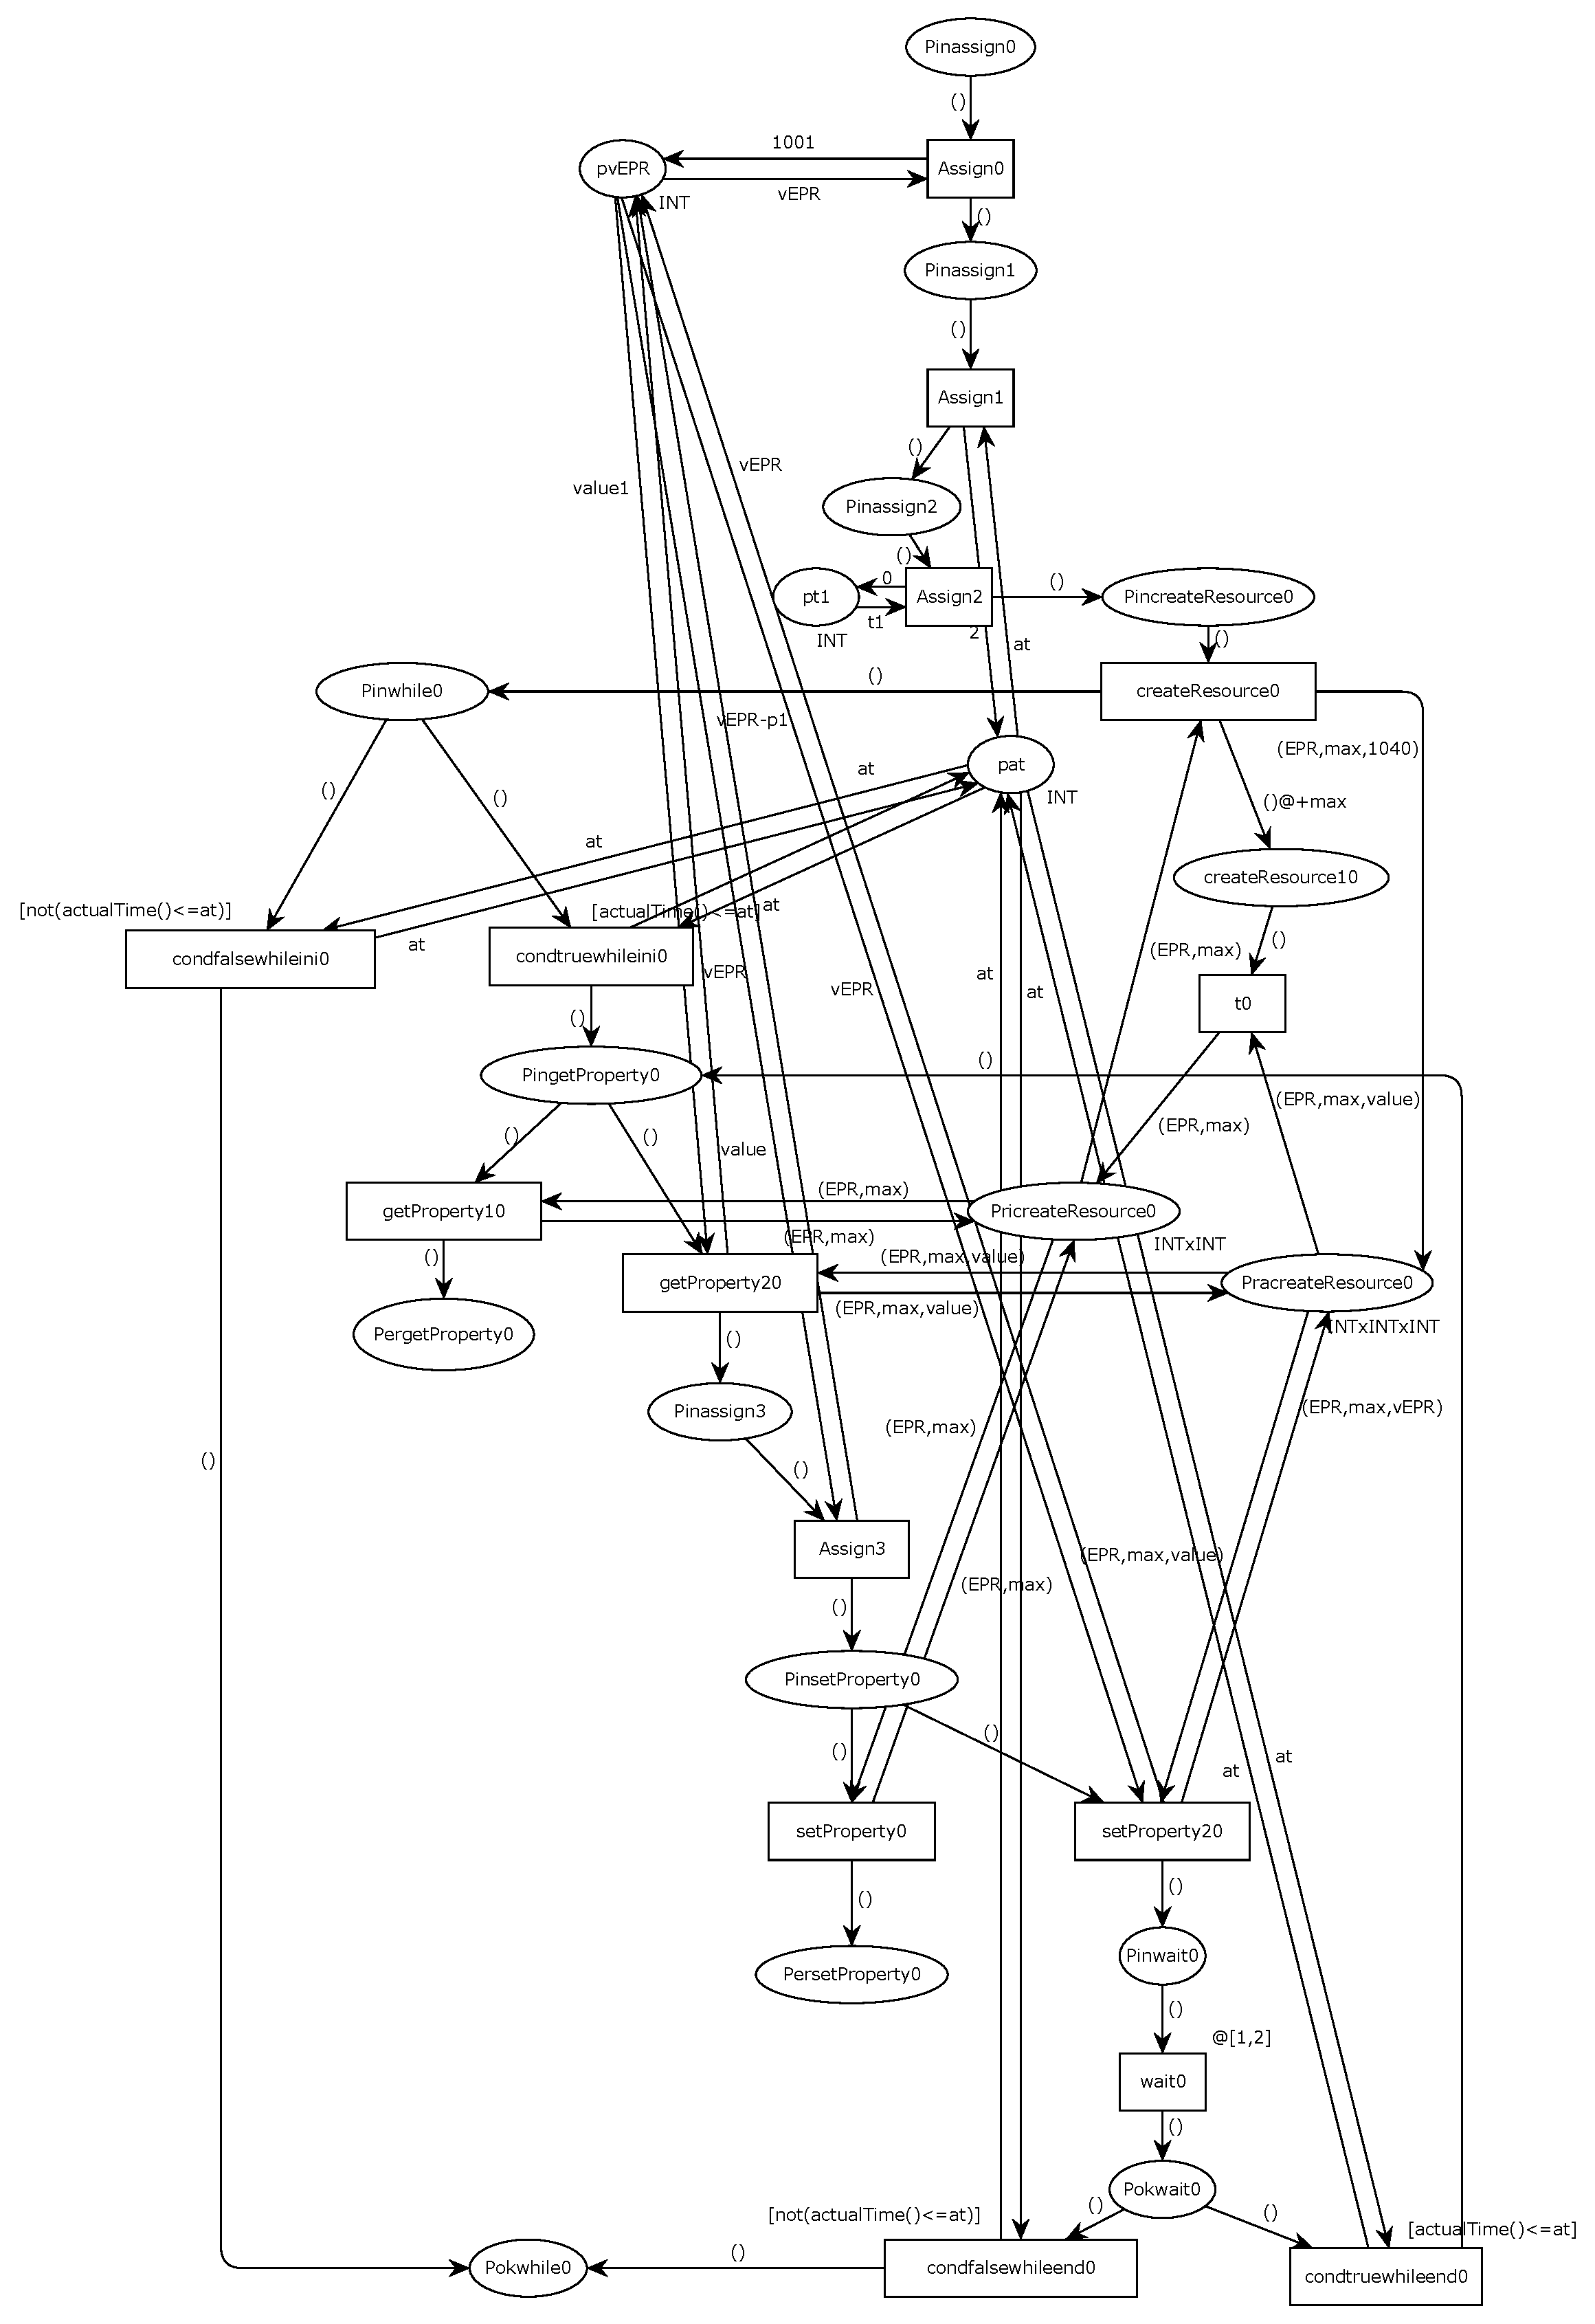
\includegraphics[width=\columnwidth, height=10cm]{Images/sistema.eps}}
\vspace{-0.4cm}
\caption{PTCPN of the online stock market.}\label{sistema}
\end{figure}
In Figs. \ref{sistema} and \ref{proceso}, the PTCPNs for one buyer and for the system are depicted.  These figures have been obtained automatically by using our tool \cite{Maria2012}. A beta version of our tool is available at \url{http://www.dsi.uclm.es/retics/bpelrf/}.
\begin{figure}[h]
\fbox{
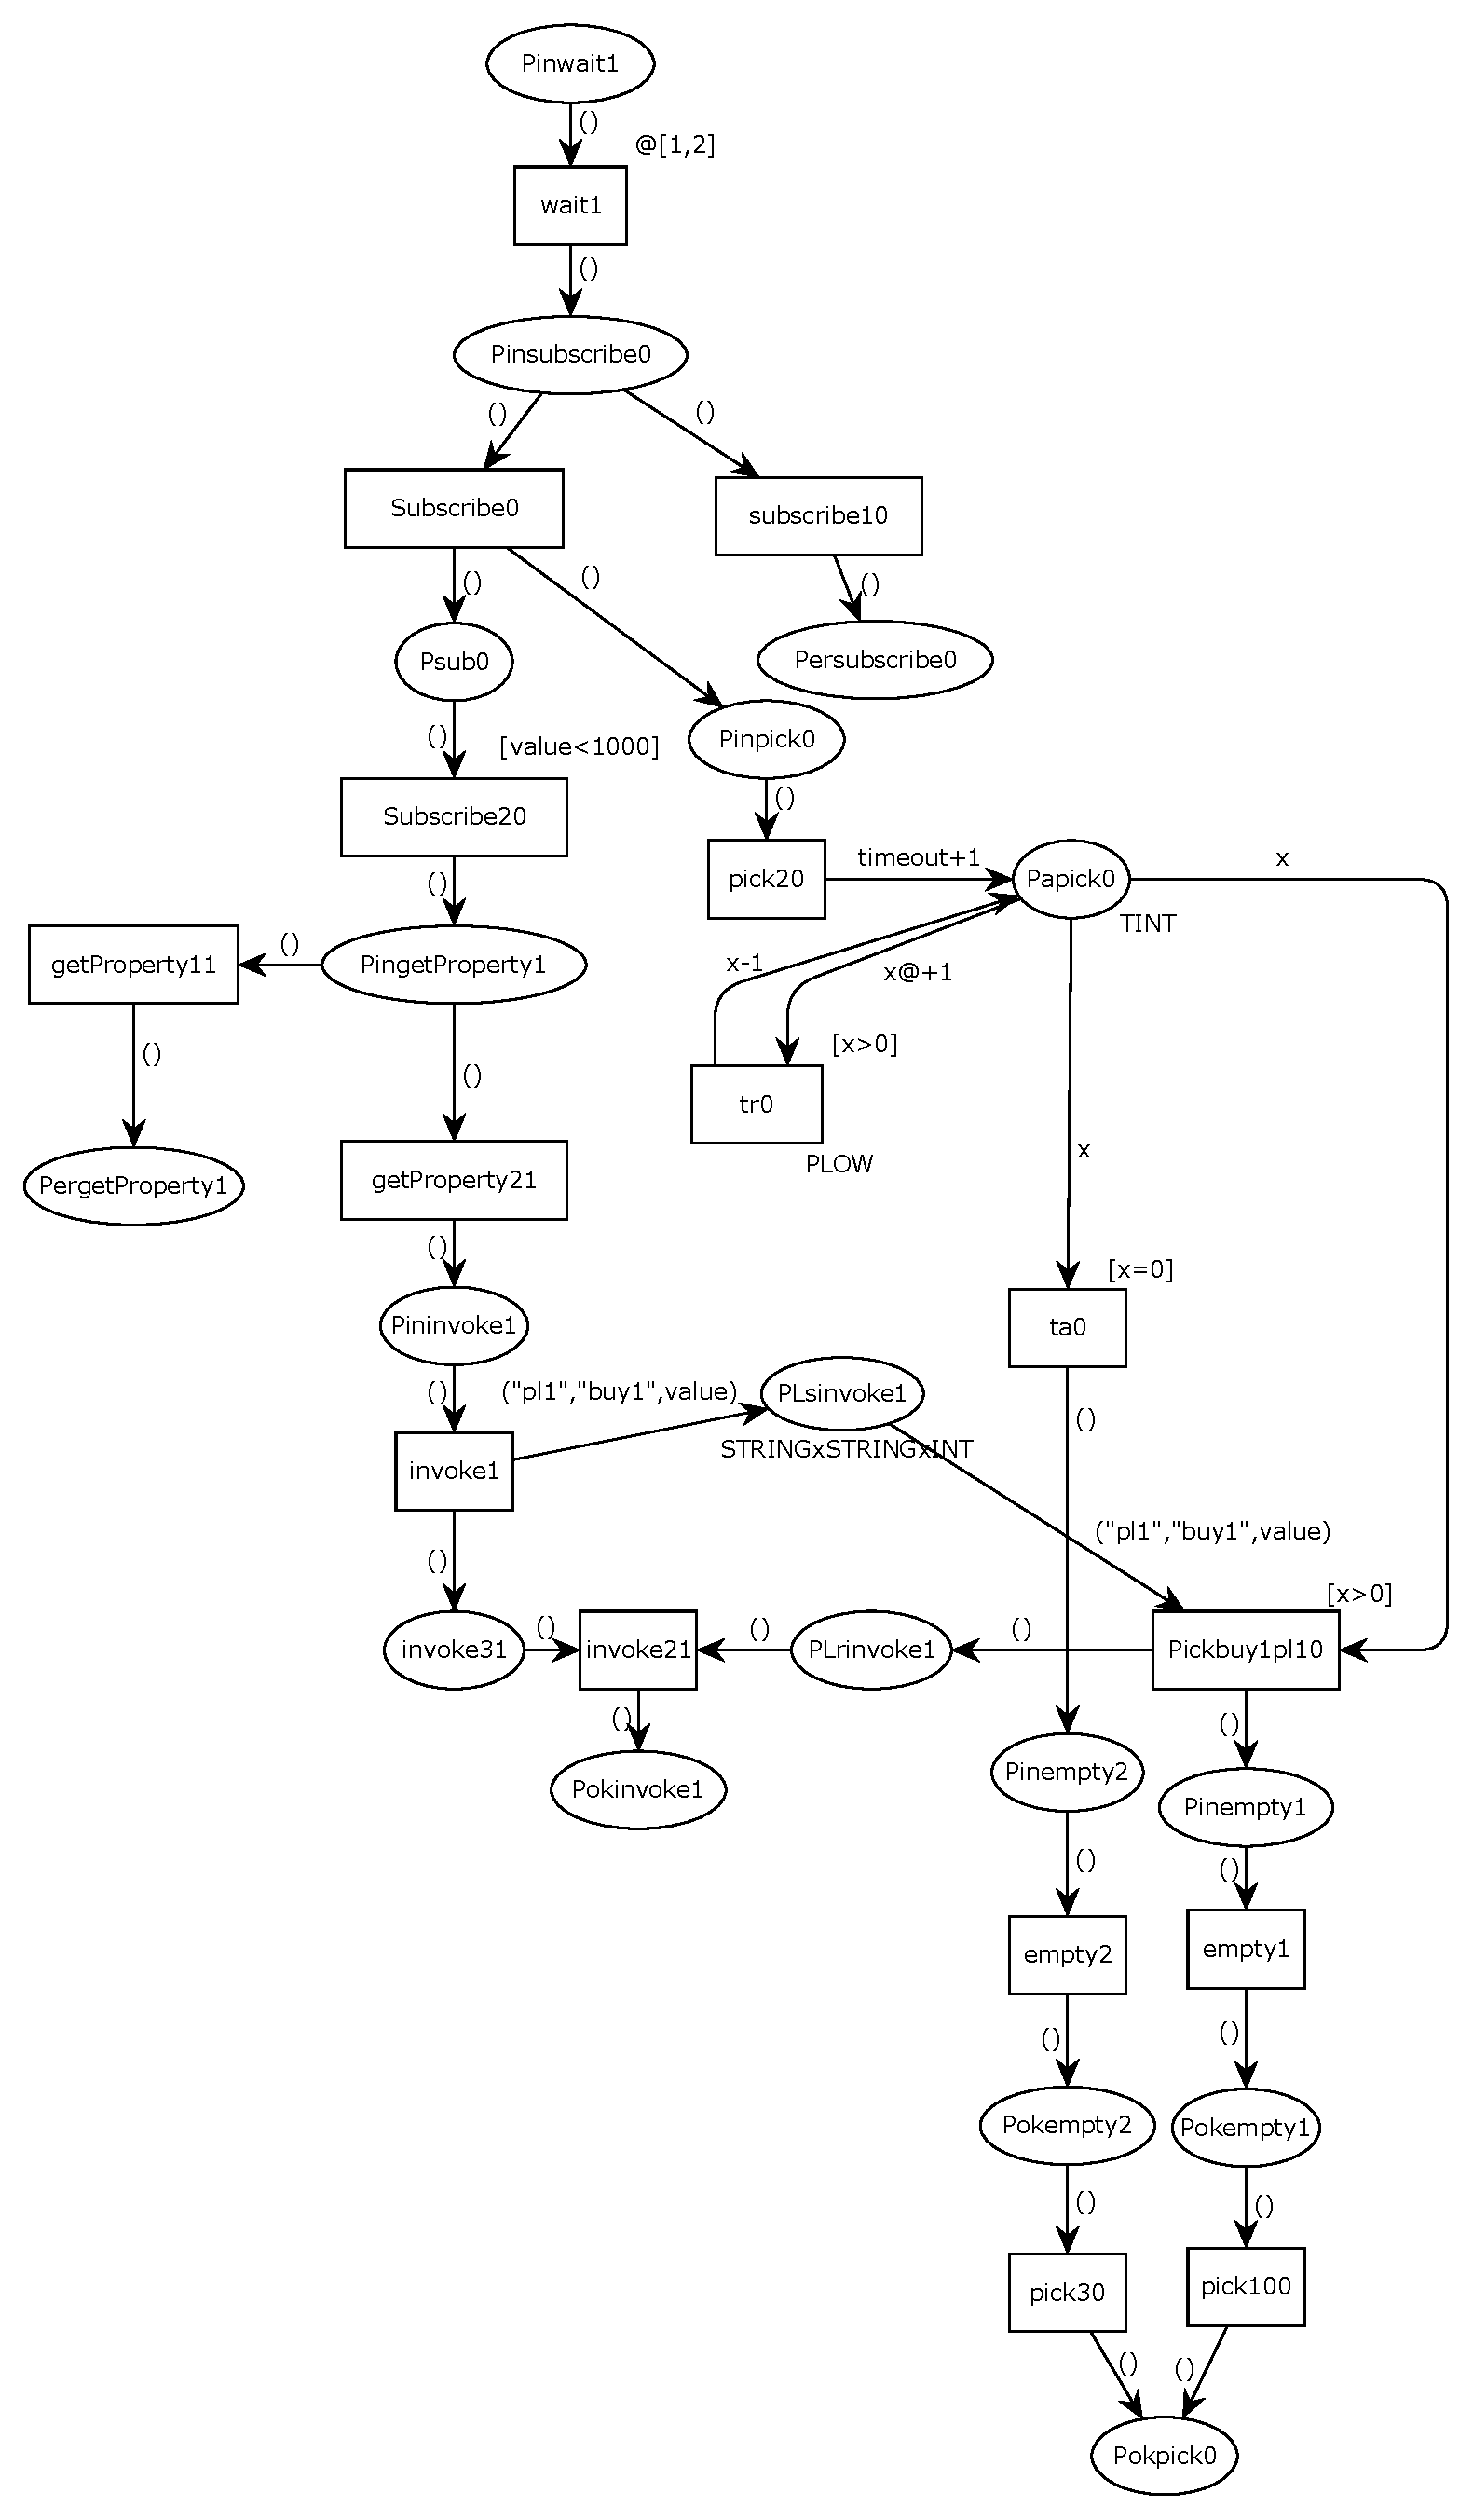
\includegraphics[width=\columnwidth, height=10cm]{Images/proceso.eps}}
\vspace{-0.4cm}
\caption{PTCPN of one buyer.}\label{proceso}
\end{figure}



\subsection{Analysis}\label{analysis}
CPNTools offers us two forms to check the correctness of our system: formal verification and simulation. 
First, the simulation helps designers to understand how the system works and it is a mean to
detect possible errors in early stages of the development process in order to refine the model according the
clients' requirements. Besides, formal verification through state space
analysis could be done in order to ensure that our system achieves some formal properties such as liveness, deadlock-freeness and so on.
In this way, Table \ref{state_space} shows the
results obtained considering 1, 2, 3, 4 or 5 investors. Note that we have considered the following assumptions:

\begin{itemize}
 \item The ``auction'' time {\em at0} is limited to 10 time units.
 \item The resource is active during 15 time units ({\em lft=15}).
 \item The resource value {\em x} is 100 money units.
 \item The value of subscription of each investor {\em i}, {\em $x_i$}, is $x-(9+i)$, that is, if the system has only one investor its subscription guard will be $x<90$, whereas with 5 investors, the last investor will have a subscription guard of $x<86$.
 \item The function {\it bid} will fluctuate the stocks price between -2 and 1 in order to simulate that the price only can rise 1 and drop 2 at most each time unit. 
\end{itemize}
We will focus on deadlock-freeness to ensure that the
system never gets stuck while the participants have activities to do
in their workflow. We have leveraged the functions offered by CPNTools
to demonstrate that in all dead markings of the system the final
place is marked, which leads us to conclude the system has finished
correctly. This final place, {\em Pokfinal0}, is marked by a transition when all the participants have finished their workflow. For the sake of clarity, we have not drawn this place in each figure. Thus, the next SML code checks when this situation
occurs: \mbox{{\small{fun DesiredTerminal n =((Mark.PetriNet'Pokfinal0
1 n) ==
1'true)}}}, \\
which returns {\em true} if the place {\it Pokfinal0} is marked. In
addition to this, it is necessary to evaluate the following predicate
to check that the list of
dead marking contains the marking of the {\em Pokfinal0} place:
\begin{center}
\mbox{{{  PredAllNodes
DesiredTerminal=ListDeadMarkings()}}}. 
\end{center}
\begin{table} [htp]
\centering
\footnotesize{
\begin{tabular}{|c|c|c|c|c|c|}
  \hline
  % after \\: \hline or \cline{col1-col2} \cline{col3-col4} ...
     & \multicolumn{5}{c|}{Number of investors}\\\cline{2-6}%\hline
  Properties     & 1 & 2 & 3 & 4 & 5 \\ \hline
  State Space Nodes & 3561  & 7569 & 16983 & 50350 & 89879 \\
  State Space Arcs & 5203 & 12843 & 33271  & 112101 &262215 \\
  Time (s) & 2 & 7 & 23 & 146 &  1140\\
  Dead Markings & 124 & 244  & 454  & 1108 &  874 \\
  \hline
\end{tabular}
}
\vspace{-0.2cm}
\caption{State space analysis results}
\label{state_space}
\end{table}
%\vspace{-0.5cm}
In Fig. \ref{queries}, we show the results offered by CPNTools to
our queries for the case of {\bf three} investors. Here, it can be
appreciated that all dead markings hold the predicate {\em DesiredTerminal}, and, therefore, when the system reaches a dead marking is because it has terminated correctly, which demonstrates the absence of deadlocks in our case study. 
%On the contrary, in Fig. \ref{RG} we can see a part of the reachability
%graph from the initial marking to a dead marking. This trace can be used for the designer to follow the path from the initial marking to the final marking in order to inspect if the system behaves according to its specification.
\vspace{-0.2cm}
%In this subsection, we are going to show the experiments conducted for the case study. CPNTools offers two ways
%to demonstrate the correctness of the system: formal verification and simulation. On the hand, the user can use
%the state space analysis tool to do formal verification
%in order to check some properties of the model such as liveness, deadlock-freeness, fairness and so on.
 %It is worthwhile to mention we will obtain more
%than one dead marking as we do not introduce in the model any
%mechanism to clean the marking of the variables, the partnerlinks,
%etc. when the final marking is reached. The solution is pretty
%straightforward, but could be a little bit tedious to draw
%transitions to reset the places when the final place is marked. As
%opposed to this, w
\begin{figure}[h]
\begin{center}%\fbox{
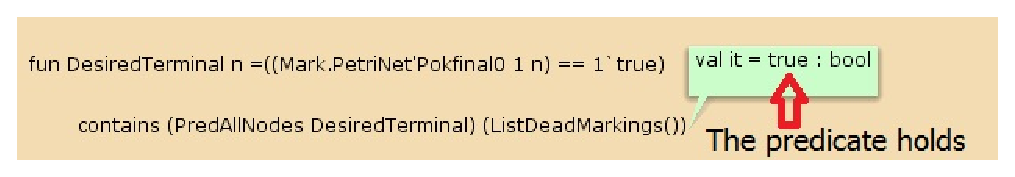
\includegraphics[width=\columnwidth,height=1.5cm]{Images/queries.eps}
\vspace{-0.7cm}
\caption{Result of the queries in CPNTools.}\label{queries}
\end{center}
\end{figure}
%\vspace{-0.7cm}
%
%\vspace{.3cm}
%
%\begin{figure}[h]
%%\fbox{
%\includegraphics[width=\columnwidth,height=6cm]{Figures/grafomarcadoscpn.eps}
%\vspace{-0.6cm}
%\caption{Partial reachability Graph (3 investors).}\label{RG}
%\end{figure}





%%%%%%%%%%%%%%%%%%%%%%%%%%%%%%%%%%%%%%%%%%%%%%%%%%
%  Conclusiones
%%%%%%%%%%%%%%%%%%%%%%%%%%%%%%%%%%%%%%%%%%%%%%%%%%
\section{Conclusions and Future Work}\label{conclu}
In this paper, we have integrated two complementary approaches in order to improve the definition of business processes models on BPEL by adding
the capability of storing their state. We have thus transformed {\em stateless} business processes into {\em stateful} business processes. To this end, we have defined a Prioritized-Timed Coloured Petri net model and presented its corresponding semantics to represent the constructions of WS-BPEL and the standards selected for the definition of resources and notifications, namely WSRF/WSN. Apart from including the notion of state in business processes, our work also includes a publish-subscribe notification system based on WS-BaseNotification, presenting a PTCPN model and its semantics. Thus, an orchestrator can show interest of being notified when a condition holds, e.g, the load of a server exceeds a certain limit. Our approach is based on the one used in CPNTools, allowing us to take advantage of its capability of analysis and verification systems. As future work, we plan to study some interesting formal properties such as safeness, soundness and so on. Furthermore, it will be also of interest to complete the semantics of WS-BPEL and WSRF/WSN by adding new features such as compensation and termination handling, and brokered notification in WSN. As regards WSRF, it seems that it could be also interesting to consider multiple
properties from different data domains, in order
to have a more realistic and usable model.
%
% ---- Bibliography ----
%
\begin{thebibliography}{10}

\bibitem{BPEL4WS}
T.~Andrews et. al.
\newblock {BPEL4WS -- Business Process Execution Language for Web Services, 
Version 1.1, 2003.\\ {\em
  http://www.ibm.com/developerworks/library/specification/ws-bpel/}}.

%\bibitem{Baldoni:2003}
%R. Baldoni, M. Contenti, S.T. Piergiovanni and A. Virgillito,
%{\em Modelling Publish/Subscribe Communication Systems: Towards a Formal Approach}.
%In IEEE International Workshop on Object-Oriented Real-Time Dependable
%Systems (WORDS), pp. 304-322, 2003.

\bibitem{Banks2006}
T. Banks, \emph{Web Services Resource Framework (WSRF) - Primer}, OASIS, 2006.


%\bibitem{Bettini2008}
% L. Bettini, R. De Nicola and M. Loreti,
% {\em Implementing Session Centered Calculi},
%In proceedings of10th International Conference COORDINATION 2008, Oslo, Norway, June 4-6, 2008. Lecture Notes in Computer Science, 5052, pg. 17-32, 2008.

%\bibitem{Bruni2011}
%R. Bruni, H. Foster, A. Luch-Lafuente, U. Montanari and E. Tuosto,
%{\em A formal support to business and architectural design for service-oriented systems}, Rigorous Software Engineering for Service-Oriented Systems, Lecture Notes in Computer Science, vol. 6582, 2011.

\bibitem{Busi:2005} N. Busi, R. Gorrieri, C. Guidi, R. Lucchi and G.
Zavattaro,
{\em Choreography and Orchestration: A Synergic Approach
for System Design}.
In International Conference of Service Oriented Computing (ICSOC),
Lecture Notes in Computer Science, vol. 3826, pp. 228-240, 2005.

%\bibitem{Busi06} N. Busi, R. Gorrieri, C. Guidi, R. Lucchi and G.
%Zavattaro.
%{\em Choreography and Orchestration Conformance for System Design}.
%In International Conference on Coordination Models and Languages (COORDINATION).
%Lecture Notes in Computer Science, vol. 4038, pp. 63-81, 2006.
\bibitem{CPNTools}
CPNTools website, \url{http://cpntools.org/}.

\bibitem{Czajkowski2004}
K. Czajkowski,  D. Ferguson, I. Foster, J. Frey, S. Graham, I. Sedukhin, D. Snelling, S. Tuecke and W. Vambenepe, \emph{The WS-Resource Framework Version 1.0}, http://www.globus.org/wsrf/specs/ws-wsrf.pdf, 2004.

\bibitem{Maria2012}
M. D\'{i}az, V. Valero, H. Macia, J. A. Mateo and G. D\'{i}az, \emph{BPEL-RF Tool: An Automatic Translation from WS-BPEL/WSRF Specifications
to Petri Nets}. In Seventh International Conference on Software Engineering Advances (ICSEA), pp. 325-330, 2012.

\bibitem{Dragoni:2009} N. Dragoni and M. Mazzara,
{\em A formal Semantics for the WS-BPEL Recovery Framework - The $pi$-Calculus Way}.
In International Workshop on Web Services and Formal Methods (WS-FM).
Lecture Notes in Computer Science, vol. 6194, pp. 92-109, 2009.

\bibitem{Dumas:2008}N. Lohmann,
{\em A Feature-Complete Petri Net Semantics for WS-BPEL 2.0}.
In International Workshop on Web Services and Formal Methods (WS-FM).
Lecture Notes in Computer Science, vol. 4937, pp. 77-91, 2008.

\bibitem{Ezenwoye:2007}
O. Ezenwoye, S.M. Sadjadi, A. Cary, and M. Robinson,
{\em Orchestrating WSRF-based GridServices}.
Technical Report FIU-SCIS-2007-04-01, 2007.

\bibitem{Farahbod:2005}
R. Farahbod, U. Gl\"asser and M. Vajihollahi,
{\em A Formal Semantics for the Business Process Execution Language for Web Services}. 
In Joint Workshop on Web Services and Model-Driven Enterprise Information Services (WSMDEIS), pp. 122-133, 2005.

\bibitem{Foster2004}
I. Foster, J. Frey, S. Graham, S. Tuecke, K. Czajkowski, D. Ferguson, F. Leymann, M. Nally, T. Storey and S. Weerawaranna, \emph{Modeling Stateful Resources with Web Services}, Globus Alliance, 2004.

\bibitem{Jensen2009}
K. Jensen and L. M. Kristensen, \emph{Coloured Petri Nets - Modelling and Validation of Concurrent Systems}, Springer, 2009.
%\bibitem{820121}
%R. Hamadi and B. Benatallah.
%\newblock {\em A {P}etri {N}et-based {M}odel for
%{W}eb {S}ervice {C}omposition.}
%\newblock In Australasian database conference, vol. 17, pp. 191-200, 2003.

%\bibitem{Kitchin2009}
%D. Kitchin, A. Quark, W. Cook and J. Misra.
%{\em The Orc Programming Language}.
%Proceedings of FMOODS/FORTE, Springer Verlag, LNCS 5522, pp. 1-25, 2009.

%\bibitem{Lapadula2008}
%A. Lapadula, R. Pugliese and F. Tiezzi,
%{\em A Formal Account of WS-BPEL}.
%Lecture Notes in Computer Science, Volume 5052, pp. 199-215,
%2008.


%\bibitem{Lapadula2007} A. Lapadula, R. Pugliese and F. Tiezzi.
%{\em Calculus for Orchestration of Web Services}. Lecture Notes in
%Computer Science, vol. 4421, pp. 33-47, 2007.


\bibitem{Leymann:2006} F. Leyman.
 {\em Choreography for the Grid: towards fitting BPEL to the resource framework}.
Journal of Concurrency and Computation : Practice \& Experience, 
vol. 18, issue 10, pp. 1201-1217, 2006.

%\bibitem{Lohman:2009} N. Lohmann, E. Verbeek, C. Ouyang and C. Stahl.
%{\em Comparing and Evaluating Petri Net Semantics for BPEL}.
%Journal of Business Process Integration and Management,
%vol. 4, issue 1, pp. 60-73, 2009.

%\bibitem{Lucchi07} R. Lucchi and M. Mazzara.
%{\em A Pi-calculus Based Semantics for WS-BPEL}.
%Journal of Logic and Algebraic Programming, vol. 70, issue 1, pp. 96-118, 2007.

\bibitem{wsfm2011} J.A. Mateo, V. Valero and G. Diaz.
{\em An Operational Semantics of BPEL Orchestrations Integrating Web Services
Resource Framework}.
In International Workshop on Web Services and Formal Methods (WS-FM), 2011.

\bibitem{Ouyang:2007} C. Ouyang, E. Verbeek, W.M.P. van der Aalst, S. Breutel, M. Dumas and A.H.M. ter Hofstede. {\em Formal semantics and analysis of control flow in WS-BPEL}.
Science of Computing Programming, vol. 67, issue 2-3, pp. 162-198, 2007.

\bibitem{Qiu:2005}Z. Qiu, S. Wang, G. Pu and X. Zhao. {\em Semantics of BPEL4WS-Like Fault and Compensation Handling}.
World Congress on Formal Methods (FM), pp. 350-365, 2005.

\bibitem{Slomiski:2006} A. Slomiski. {\em On using BPEL extensibility
to implement OGSI and WSRF Grid workflows}.
Journal of Concurrency and Computation : Practice \& Experience,
vol. 18, pp. 1229-1241, 2006.

\bibitem{Wirsing2011bis}
M. Wirsing and M. Holzl (Eds.),
{\em Rigorous Software Engineering for Service-Oriented Systems}, 
Lecture Notes in Computer Science, Vol. 6582. Springer-Verlag, 2011.

\bibitem{wsaddressing}
\newblock {Web Services Addressing (WS-Addressing), 
\\ {\em
  http://www.w3.org/Submission/ws-addressing/}}.
%\bibitem{Wirsing2011}
%M. Wirsing, R. De Nicola, S. Gilmore, M. Holzl, R.
%Lucchi, M. Tribastone and G. Zavattaro
%{\em Core Calculi for Service-Oriented Computing}, 
%Rigorous Software Engineering for Service-Oriented Systems, Lecture Notes in Computer %Science, vol. 6582, 2011.

%\bibitem{W3C}
%World Wide Web~Consortium (W3C).
%\newblock {{\em http://www.w3.org/}}.

%\bibitem{WSCDL}
%Web Services Choreography Description Language Version 1.0 (WS-CDL).
%\newblock {{\em http://www.w3.org/TR/ws-cdl-10/}}.

\end{thebibliography}
\end{document}